%!TEX root = ../thesis.tex
%*******************************************************************************
%****************************** Fourth Chapter **********************************
%*******************************************************************************

\chapter{Epidemiological and genetic characterisation of perianal Crohn's Disease}

% **************************** Define Graphics Path **************************
\ifpdf
    \graphicspath{{Chapter4/Figs/Raster/}{Chapter4/Figs/PDF/}{Chapter4/Figs/}}
\else
    \graphicspath{{Chapter4/Figs/Vector/}{Chapter4/Figs/}}
\fi
\section{Contributions}
Genotype and imputation quality control was performed by Dr. Laura Fachal and kinship analysis was performed by Dr. Marcus Tutert as part of the ongoing International IBD Genetics Consrtium GWAS project that is being undertaken in the Anderson laboratory. HLA allele imputation was performed by Dr. Qian Zhang as part of his IBD-BR drug response and disease progression study. I performed all the GWAS analyses, meta-analyses and all downstream analyses described in this chapter.
\section{Introduction}
Perianal Crohn's disease (pCD) is a sub-phenotype of Crohn's disease, a chronic inflammatory disease of the gut that affects 1\% of the population worldwide. pCD represents a major burden on both patients and healthcare providers, and is estimated to affect 20-40\% of CD patients worldwide, with a higher prevalence in Asia than in Western countries \cite{Ng2016-al}. As their disease progresses, CD patients become more likely to develop perianal symptoms. Twenty years after their CD diagnosis, CD patients have a 32\% cumulative probability of developing pCD \cite{Brochard2022-hx}. Timing of pCD diagnosis, however, varies significantly between healthcare systems. Previous studies from countries including France, Sweden and Japan have reported that between 4\%-68\% of pCD patients present with perianal symptoms before or at the time of CD diagnosis \cite{Mizushima2021-hk,Pogacnik2019-aj,Wils2021-ao}.\\

\subsubsection{Clinical picture of pCD}
pCD patients present with a variety of perianal symptoms. These include perianal skin tags, fissures, ulcers, faecal incontinence, rectal discharge and bleeding, perianal abscess, and fistulas. Perianal fistulas are the most common form of pCD, followed by perianal abscess \cite{Eglinton2012-vx}. Likewise, the impact of pCD on patients is multi-faceted. In addition to physical manifestations, patients report impaired quality of life as well as social and emotional complications of pCD. Furthermore, surgical interventions that aim to treat pCD and restore normal ano-rectal functions, such as seton insertion and fistula drainage, often impact essential functions such as walking and sitting \cite{Adegbola2020-nd}. Moreover, pCD patients, who often require multiple surgical interventions, suffer from high recurrence and relapse rates of pCD. In fact, only one third of pCD patients are estimated to achieve remission \cite{Panes2018-su,Braithwaite2017-zo}. \\

% To inform clinical decision making, several clinical scoring systems have been proposed to describe the clinical picture and predict prognosis of pCD. The first pCD scoring system was published by Hughes in 1992 \cite{Hughes1992-kc}. Hughes classified pCD lesions into primary lesions, such as fissures and ulcers, and secondary lesions such as skin tags, abscess and fistulas \cite{Safar2007-dk}. A numeric score was given based on the presence and severity of ulcerations, fistulas or abscess, and strictures. However, this classification has had limited impact on clinical practice \cite{Scheurlen2023-gk}. The Perianal Disease Activity Index is the  (PDAI), which has been devised to predict surgical outcomes in pCD patients, is the most widely used measure of pCD activity. PDAI scores six pCD clinical indicators on a Likert score: abscess, fistula, fissure and ulcer, stenosis, incontinence, and concomitant disease. Patients with no perianal involvement score 0 and patients with advanced perianal disease score a maximum of 55  \cite{Pikarsky2002-gf}. Compared to other clinical scoring systems, PDAI correlates well with pCD outcome and has been recommended for use in clinical practice \cite{Irvine1995-ej}.\\

Despite the diversity in presentation and course, pCD patients share a number of Crohn's disease characteristics. pCD is  more common among patients with more distal than proximal disease, and patients with colonic or rectal CD are more likely to develop or initially present with pCD. Moreover, pCD tends to drive Crohn's disease towards a more invasive behaviour. Initially, two thirds of patients have inflammatory manifestations, but over time, the majority of pCD patients display increasingly stricturing and penetrative characteristics of CD \cite{Peyrin-Biroulet2010-mf,Scharl2017-sp}, which are characterised by a narrowing of the lumen, and development of abdominal fistulas, inflammatory masses and abscess \cite{Gasche2000-qh}.  However, invasive distal CD does not always precede pCD, which can sometimes present a diagnostic challenge in clinical settings. Although 95\% of patients will eventually develop luminal disease, an estimated 17.2\% of patients initially present with pCD only \cite{Eglinton2012-hh}. \\


\subsubsection{Pathogenesis of pCD}
At a more fundamental level, our biological understanding of pCD fistula formation and progression mechanisms is still markedly lacking. One proposed pathophysiological mechanism is epithelial-to-mesenchymal transformation (EMT). EMT is a well-studied biological process, whereby polarised epithelial cells gain mesenchymal functions, such as enhanced cell invasion, and migration (reviewed in \cite{Kalluri2009-uu}). The EMT hypothesis is supported by the presence of transitional cells which express both epithelial and mesenchymal cell markers in fistula tracts. These include epithelial markers cytokeratin 8 and 20, and mesenchymal markers vimentin and actin. Transforming growth factor $\beta$ and interleukin-13, which have been associated with the initiation of EMT, have also been identified in transitional cells lining pCD fistula tracts \cite{Scharl2013-uf,Bataille2008-ej,Bataille2004-vf}. Despite these observations, little is understood about the causal biology of pCD. What are the drivers of this transformation? What causes variation in fistulising disease severity? Which biological pathways give rise to fistulas and what facilitates their development into complex branching structures? What is the role of genetic variation in pCD predisposition? In this regard, genome-wide association studies have improved our understanding of the pathophysiology of several complex disease \cite{Cano-Gamez2020-nm}. In the case of pCD, a well-powered GWAS between CD patients who develop pCD and CD patients who do not can help us understand which effector genes and biological pathways are causally linked to pCD risk. Unfortunately, none of the pCD GWAS conducted so far were able to identify genome-wide significant variants associated with pCD risk. Some studies have investigated nominally significant association to better understand pCD biology, but the hypotheses about causal biology remain difficult to reconcile. For example, based on a GWAS of 1,720 CD patients with and without pCD, Kaur et al. \cite{Kaur2016-bs} report an enrichment of nominally-associated variants in genes implicated in the JAK/STAT pathway, a proinflammatory signalling cascade that has previously been implicated in several autoimmune diseases \cite{Hu2021-us,Seif2017-bk}. More recently, Akhlaghpour et al. \cite{Akhlaghpour2023-jw} found a nominally-associated coding variant that impaired macrophage phagocytosis, and hypothesised that it may contribute to the pathogenesis of fistulising pCD. But overall, there is no clear consensus on the genetic underpinnings of pCD risk.\\

\subsubsection{Available pCD cohorts}
The NIHR IBD-BR is a UK-wide collaborative project that is part of the NIHR Bioresource, with the aim of recruiting 50,000 patients with Crohn's disease, ulcerative colitis or unclassified IBD. The IBD-BR collects phenotypic and epidemiological information (both clinical and self-reported) as well as DNA samples for both array genotyping and whole-genome and whole-exome sequencing. The aims of the IBD-BR are wide-ranging. These aims include understanding the genetics of IBD response to therapy, disease mechanism as well as determinants of disease course \cite{ibdbr-protocol-v8,ibdbr-questionnaire-v7,ibdbr-further-info}. So far, the IBD-BR has recruited over 31,000 patients, with epidemiological characteristics, clinical phenotypes, extra-intestinal manifestations, prescribed medications and treatment history, surgical history and disease behaviour and complications. The recruitment process starts by an expression of interest by volunteers who visit participating recruitment centres. Interested volunteers are then provided with an invitation letter and a patient information sheet that provides information on study requirements. Patients who agree to take part are then provided with an informed consent form, and subsequently asked to complete a health and lifestyle questionnaire. After these initial steps, the clinical team then proceeds to collect clinical data from hospital records. A clinician or research nurse extracts core information including IBD type, location and behaviour, complications, comorbidities, family history, smoking history, surgical data and
drug therapy outcomes \cite{ibdbr-protocol-v8}. Disease location data include details of perianal manifestations, which can be used to define a pCD case-control cohort.\\

Another pCD case control cohort can be defined using data from The UK IBD Genetics Consortium (UKIBDGC), a large collaborative consortium that studies the genetics of IBD susceptibility, progression and drug response. Patients are recruited from multiple UK centres in Cambridge, Edinburgh, Manchester, Newcastle, Exeter, Oxford, London, Dundee and Nottingham, and other sites across the UKB \cite{ukibdgc-info}. In additiona to basic epidemiological data such as sex, age, smoking and family history, data on type of IBD, location, surgery, and extraintestinal manifestations is recorded. Disease location data also include whether the disease is located in the perianal region.\\

Although data on perianal disease are recorded for both cohorts, the depth of clinical phenotyping is different. For example, the IBD-BR, contains information about specific manifestations of pCD. Clinicians and clinical nurses who complete the IBD-BR questionnaire perform an automated search of hospital records for clinical IBD information, including perianal manifestations \cite{ibdbr-protocol-v8}.  If the search is unsuccessful, they ask patients about perianal involvement: \textit{"Ever had perianal involvement? 1) Yes 2) No 3) Unknown"}  and record the answer in the clinical questionnaire \cite{ibdbr-questionnaire-v7}. A follow-up question about the type of perianal involvement is then asked: \textit{“If Yes - What type of perianal lesion has the patient had? (Select all that apply): 1) Tags/fissures/ulcers 2) Perianal abscess 3) Simple fistula 4) Complex fistula 5) Other”}. Clinicians may report one or more perianal involvement manifestations.  Unlike IBD-BR, the specific manifestations of pCD , such as fissures, ulcers or fistulas are not recorded for UKIBGC participants and only a binary phenotype is recorded (pCD+ or pCD-). \\

In this chapter, I describe several analyses I conducted to characterise pCD. Using the rich clinical phenotyping in the IBD-BR, I first explored the clinical characteristics of pCD+ patients, which largely conformed with what is known about the disease characteristics of pCD. Moreover, given our limited understanding of the genetic underpinnings of pCD \cite{Eglinton2012-ls,Latiano2009-bu,Tozer2009-mp,Akhlaghpour2023-jw,Kaur2016-bs}, I also performed a pCD GWAS meta-analysis leveraging the pCD cohorts of IBD-BR and UKIBDGC to identify pCD-associated variants. I conclude with an analysis that may partly explain the discovered pCD-associated hit and outline future steps for a more comprehensive understanding of the genetic underpinnings of pCD.
\section{Methods}
\subsection{pCD prevalence estimates}
IBD-BR patients were diagnosed with CD over several decades, mostly from 1980 till 2018. To investigate the temporal trends of pCD prevalence, I divided participants by year of CD diagnosis into 39 windows, and calculated pCD point prevalence in each two-year period. Additionally,to calculate 95\% confidence intervals around each point estimate, I randomly subsampled CD patients 1,000 times using a bootstrap proceducre implemented in the \Verb+boot()+ functions. Finally, I compared overall trends in prevalence estimate by pooling CD participants diagnosed with CD before and after 2010 and calculated point estimates and confidence intervals as mentioned before. The difference between these overall estimates was then tested using a t-test to deterime if pCD prevalence has significantly decreased before and after 2010.
\subsection{UK IBD Genetics Consortium Genotype Quality Control}
UKIBDGC samples were genotyped with two genotyping arrays: Affymetrix Human Mapping 500K Array (I will refer to this as GWAS1; number of variants before QC=469,281), and Illumina Human Core Exome-12v1.0 or its newer version Illumina Infinium Core Exome-24v1.1 (I will refer to this as HCE; number of variants before QC=535,434 and 557,662 respectively). Quality control for UKIBDGC genotype data was performed as part of the International IBD Genetics Consortium cases-control meta-analysis. QC was performed using a combination of Plink (v1.9 and v2), bcftools (v1.16), and KING (v2.2.4).
\subsection{Variant-level QC}
Variants that met the following criteria were excluded: 
\begin{itemize}
  \item Low call rate (< 0.95 for variants with minor allele frequency (MAF) $>$ 0.01 or $<$ 0.98 for variants with MAF $\leq$ 0.01).
  \item Significant difference in genotype call rate (P-value $< 10^{-4}$) between IBD cases and controls.
  \item Large allele frequency (AF) differences between UKIBDGC and Gnomad (Non-Finnish Europeans), or TOPMed (global) using the following formula:

$$\frac{(P_{1}-P_{0})^{2}}{(P_{1}+P_{0})(2-P_{1}-P_{0})} > \epsilon$$ 


where $\epsilon=0.025$ or $0.125$, for Gnomad and TOPmed respectively,  $P_{0}$ is the minor allele frequency (MAF) in Gnomad or TOPMed and $P_{1}$ is UKIBDGC MAF. This formula accounts for larger AF differences between UKIBDGC and population references in common than in low-frequency variants. The TOPMed global AF difference cutoff is higher to account for AF computed across diverse populations
\item Hardy Weinberg Equilibrium (HWE) P-value < $10^{-5}$ in IBD controls or < $10^{-12}$ in IBD cases.
 or 
\item Monomorphic variants. 
\end{itemize}

\subsection{Sample-level QC}
Samples that meet the following criteria were excluded:
\begin{itemize}
\item Missing genotyping rate $>$ 0.05
\item Heterozygosity estimate $\pm$ 4 standard deviations from the European-ancestry mean, or 
\item mismatch between recorded gender and genotypically-inferred sex. 
\end{itemize}
\subsection{Imputation to TOPMed}
The TOPMed imputation server (imputationserver at 1.5.7) was used for UKIBDGC genotype imputation. Alleles at directly genotyped variants with an empirical imputation $R < -0.5$ were flipped, and variants with empirical $R^{2} \leq 0.5$ were excluded after imputation. After their exclusion, imputation was repeated, and another HWE filtering step was performed.

\subsection{IBD-BR Genotype QC and Imputation}
The cohort was genotyped with two different versions of the UKBiobank ThermoFisher genotyping array. The same genotype QC steps as UKIBDGC were applied to IBD-BR, except for 1) The AF difference check, where 1000 Genomes Panel (1000GP) was used as a reference panel 2) Imputation, where the Sanger Imputation Server was used \cite{1000gp}, with two imputation reference panels: UK10K+1000GP and HRC. Imputed genotypes from both panels were combined. For variants that existed in both panels, HRC imputed genotypes were retained. 

Genotypic principal components (PC) were estimated for all participants, using a set of genotyped variants that were also available in the 1000 Genomes Project (100GP; excluding variants associated with IBD susceptibility; P-value < $10^{-4}$, and variants in long LD regions (as defined in \cite{plink_high_ld}). This final list was pruned with the following parameters: window size = 50 kbp; step size = 5; $R^{2}$ = 0.2. PCs were then projected to 1000GP PCs. Samples within the European ancestry group were retained for the subsequent analyses. 

\subsection{Identification of overlapping samples between UKIBDGC and IBD-BR}
Identification of duplicate individuals between UKIBDGC and IBD-BR genotyping data was performed with KING \cite{king-software}. Duplicates were defined as sample pairs with a kinship coefficient > 0.354 as recommended in KING documentations \cite{king-software}. Estimation of kinship coefficient was performed using post-QC genotyped SNPs (number of variants used for kinship inference between IBD-BR and GWAS1=42,292:, and between IBD-BR and HCE=53,431).

\subsection{Genome-wide association analysis}
All genome-wide association analyses were performed using REGENIE v3.2.5 \cite{Mbatchou2021-qm} following a 2-step approach. This approach is more computationally efficiency than other approaches that account for cryptic relatedness between individuals, such as linear mixed models. Briefly, in step 1, a whole-genome regression model is fitted using a subset of high-quality genome-wide variants in order to estimate a set of genome-wide predictors that capture a large fraction of phenotypic variance. These predictors are then included as covariates in the single-variant association models tested in step 2, where a larger set of variants of interest are tested for association. I used post-QC genotyped variants in step 1 as recommended by REGENIE documentation ($N_{IBD-BR}$=338,697; $N_{UKIBDGC(HCE)}$=359,209; $N_{UKIBDGC(GWAS1)}$=436,931), and both genotyped and imputed variants in step 2, testing all autosomal chromosomes ($N_{IBD-BR}$=9,777,139; $N_{UKIBDGC(HCE)}$=,916,200; $N_{UKIBDGC(GWAS1)}$=8,897,554). The step 2 model was specified as following: pCD $\sim$ variant + sex + genotypic PCs, using first 4 genotypic PCs. Step 2 reports single-variant association summary statistics. 

\subsection{Meta-analysis of IBD-BR and UKIBDGC cohorts}
I used METAL to perform the fixed-effects meta-analysis between the IBD-BR and UKIBDGC summary statistics.  METAL can perform fixed-effects meta-analysis using one of two different well-established schemes: P-values and effective sample size, or effect sizes and standard errors. The P-value scheme is implemented to enable meta-analysis of GWAS summary statistics that do not report the effect allele, while the effect sizes scheme can be used when each variant's effect size and effect allele are reported. All my pCD GWAS analyses report the effect allele, so I used the effect size scheme of METAL (\Verb+SCHEME STDERR+). \\

There was a total of 8,473,930 overlapping variants across the meta-analysed summary statistics, and an additional 1,645,123 variants that were unique to one of the studies, 42.7\% of which were indels. Given that 16\% of variants were unique to one of cohorts, I did not remove them from their respective summary statistics file. It is important to note, however, that this choice may favour variants that are available in all studies. 

\begin{table}[H]
  \caption{Number of SNPs and indels in each of the three GWAS summary statistics.}
  \centering
  \begin{tabular}[t]{lrrr}
  \toprule
  \textbf{Studies} & \textbf{SNP} & \textbf{Indel} & \textbf{Total}\\
  \midrule
  IBD-BR & 8,626,072 & 1,150,933 & 9,777,005\\
  UKIBDGC (GWAS1) & 8,307,857 & 589,198 & 8,897,055\\
  UKIBDGC (HCE) & 8,325,721 & 589,997 & 8,915,718\\
  \bottomrule
  \end{tabular}
  \end{table}

Moreover, METAL automatically aligns any variants that may be flipped between the meta-analysed summary statistics. METAL also enables filtering of variants to be meta-analysed based on their allele frequencies, which was not necessary since I previously filtered out variants with MAF < 0.01 in each summary statistics file. Finally, given the potential subpopulation stratification in the IBD-BR GWAS ($\lambda_{GC}$=1.08), I enabled a METAL option to correct genomic inflation before performing the meta-analysis (\Verb+GENOMICCONTROL ON+) as recommended in METAL's documentation website. There was no evidence of genomic inflation in the meta-analysed summary statistics ($\lambda_{GC}$=1.03).\\

For each variant, METAL outputs the effect allele, meta-analysed effect size, standard error, and P-values. After performing meta-analyses, it is important to compare the effect sizes between the meta-analysed cohorts. Comparison of both the direction and magnitude of effect sizes gives an indication on how similar the estimated effects of meta-analysed genetic variants are. To formally test this, I used Cochran's Q test of effect size heterogeneity implemented in METAL. Cochran's Q test asseses two or more effect size estimates and their corresponding standard errors and reports a $\chi^{2}$ statistic that quantifies the deviation from the null hypothesis that the meta-analysed effect sizes are similar. Depending on the number of meta-analysed studies (in this case 3), a P-value is derived from a theoretical $\chi^{2}$ distribution with $N-1$ degrees of freedom, where N is the number of meta-analysed studies (heterogeneity of effect P-value $P_{het}$). I used $P_{het}$ to test if the genome-wide significant variants demonstrate heterogeity of effect size between the meta-analysed cohorts. To account for multiple variants being tested, I set a Bonferroni-corrected P-value threshold for rejecting the null hypothesis (P-value < $\frac{0.05}{k}$, where $k$ is the number of variants tested).

% \subsection{Post-hoc power analysis of genome-wide significant variants}
% Power analysis was conducted to verify if genome-wide significant variants were expected given the meta-analysis sample size. I used the R package \Verb+genepwr+ v1.04 \cite{genepwr-docs} to calculate the power of the study to detect each genome-wide significant variant given each variant's effect size, the study sample size, and case proportion over a range of MAFs from 0.01 to 0.1, and assuming a significance level $\alpha < 5\times10^{-8}$.


\subsection{LD calculation from 1000GP}
Reference LD panels obtained from the 1000 Genomes Project High Coverage project \cite{1000gphc} were used in the post-GWAS check to study the relationship between LD and association strength at the genome-wide significant locus. $R^{2}$ values were calculated between the index variant and all variants in the locus. I downloaded VCFs from the 1000GP high coverage and used PLINK v1.9 to compute LD between all variants and the index variant in a 1mbp window. I used unrelated individuals with non-Finnish European ancestry (NFE; N=426). Relevant samples were included in the LD calculation using the following PLINK command:
\begin{verbatim}
  plink --r2 --keep EUR.samples --ld-window-r2 0 
\end{verbatim}

\subsection{$\chi^{2}$ comparison between different pCD definitions}
In order to compare association statistics from the pCD meta-analysis to meta-analyses performed using more severe pCD+ case criteria (all perianal manifestations, abscess and fistula only, fistula only and complex fistula only), I adjusted the broad-definition $\chi^{2}$ values using this formula:

 $$\chi^{2}_{Broad,n}=\frac{n}{N}\chi^{2}_{Broad}$$

where $n$ is the sample size of the meta-analysis being assessed, $\chi^{2}_{Broad}$ is the broad-definition observed association statistic and  $\chi^{2}_{Broad,n}$ is the broad-definition association statistic adjusted for sample size. This adjustment ensure that comparison of association statistics from meta-analyses with different sample sizes is valid.

%From script:
%/nfs/users/nfs_o/oe2/ibdbr/scripts/hla/cond_meta.R

\subsection{HLA allele imputation}
HLA genes located in the major histocompatibility complex region (MHC) are known to contribute to immune disease susceptibility \cite{Shiina2009-wt}. Although sequence-based typing (SBT) is the gold standard to identify HLA alleles, its relatively higher cost and the complexity of HLA sequencing has prevented scaling up of SBT methods to large cohorts \cite{Beksac2014-gm}. HLA allele imputation methods based on SNP arrays are a reliable alternative to SBT methods of HLA typing, and can be performed using a small number of genotyped SNPs in each HLA gene \cite{De_Bakker2006-ho,Monsuur2008-fk,Jia2013-mh,Zheng2014-mj,Cook2021-px,Naito2021-jl} (reviewed in \cite{Naito2022-qy}). \\

HLA alleles were imputed for all IBD-BR and UKIBDGC individuals using HIBAG, a computationally efficient prediction algorithm that was pre-trained on a diverse set of haplotypes from different ancestries and is used to impute HLA alleles \cite{Zheng2014-mj}. Model parameters that were pre-trained on SNPs from the UK Biobank Affymetrix Axiom array from European and multi-ethnic ancestries were used in HLA imputation (downloaded from \cite{hibag-models-docs}). After downloading the pre-trained models, HLA imputation was performed at the HLA allele and HLA allele group levels  for a total of 7 HLA genes (4-digit and 2-digit resolutions; Table \ref{table:hla_allele_num}). 

\begin{table}[H]
  \centering
  \caption{Number of genotyped variants used to perform HLA imputation.}
  \label{table:hla_allele_num}
  \begin{tabular}{|l|l|l|}
  \hline
  Gene     & 2 digits & 4 digits \\ \hline
  HLA*A    & 723      & 717      \\ \hline
  HLA*B    & 763      & 752      \\ \hline
  HLA*C    & 819      & 770      \\ \hline
  HLA*DPB1 & 478      & 478      \\ \hline
  HLA*DQA1 & 753      & 655      \\ \hline
  HLA*DQB1 & 754      & 702      \\ \hline
  HLA*DRB1 & 675      & 653      \\ \hline
  \end{tabular}
  \end{table}
For each HLA allele, I performed the association test using the logistic regression model: pcd status $\sim$ HLA allele copies + covariates, with the R function \Verb+glm(family=binomial())+ and using the same covariates as used in the GWAS. The association analysis were performed separately for each of IBD-BR, UKIBDGC (HCE) and UKIBDGC (GWAS1). The association effect sizes and standard errors were subsequently meta-analysed using the R package \Verb+metafor+. Additionally, I performed conditional association analysis to investigate if any HLA alleles can account for genome-wide significant SNPs. Conditional association analyses were performed by including SNP dosages as covariates in the same model. 
% \subsection{First subsection in the first section}
% \dots and some more 

% \subsection{Second subsection in the first section}
% \dots and some more \dots

% \subsubsection{First subsub section in the second subsection}
% \dots and some more in the first subsub section otherwise it all looks the same
% doesn't it? well we can add some text to it \dots

% \subsection{Third subsection in the first section}
% \dots and some more \dots

% \subsubsection{First subsub section in the third subsection}
% \dots and some more in the first subsub section otherwise it all looks the same
% doesn't it? well we can add some text to it and some more and some more and
% some more and some more and some more and some more and some more \dots

% \subsubsection{Second subsub section in the third subsection}
% \dots and some more in the first subsub section otherwise it all looks the same
% doesn't it? well we can add some text to it \dots

\section{Results}
Among 30,894 IBD-BR participants, 15,152 were diagnosed with Crohn's disease, 14,819 of which had perianal involvement data: 4,448 answered "\textit{Yes}" to “\textit{Ever had perianal involvement?}” (pCD+; 30\%), 9,751 answered "\textit{No}" (pCD-; 65.8\%), and 620 answered “\textit{Unknown}” (4.1\%), matching previous pCD prevalence estimates. Perianal simple or complex fistula was the most common manifestation (2327;  52.3\% pCD+ participants), followed by perianal abscess (1806; 40.5\% of pCD+ participants).

From 26,327 UKIBDGC patients, a total of 8,977 were diagnosed with CD. 7106 CD patients had perianal involvement information. pCD prevalence was lower than IBD-BR. 18.2\% of CD patients reported perianal disease location, 61\% reported a different disease location, and 20.8\% answered "\textit{Unknown}". UKIBDGC does not report specific manifestations of pCD.

\subsection{Epidemiological characteristics}
Epidemiological characteristics of pCD+ and pCD- patients were largely similar in both cohorts (Table \ref{table:epidem}). Males were more likely than females to report perianal involvement in both cohorts (P-value={$7\times10^{-4}$} and {$8\times10^{-6}$} in IBD-BR and UKIBDGC respectively). pCD+ was not associated with a family history of CD, while smoking was slightly less common in pCD+ patients (P-value=0.006 and 0.003).
\setlength{\tabcolsep}{10pt} 
\renewcommand{\arraystretch}{1.5}
\begin{table}[H]
  \caption{Epidemiological characteristics of pCD+ and pCD- patients in IBD-BR and UKIBDGC}
  \label{table:epidem}
  \centering
  \begin{tabular}[t]{lllll}
  \toprule
  \multicolumn{1}{c}{ } & \multicolumn{2}{c}{IBD-BR} & \multicolumn{2}{c}{UKIBDGC} \\
  \cmidrule(l{3pt}r{3pt}){2-3} \cmidrule(l{3pt}r{3pt}){4-5}
   & pCD+ & pCD- & pCD+ & pCD-\\
  \midrule
  Male & 2115 (47.5) & 4339 (44.5) & 807 (49.5) & 2363 (43.2)\\
  Female & 2333 (52.5) & 5412 (55.5) & 824 (50.5) & 3112 (56.8)\\
  Family History & 1325 (34.7) & 2795 (34.2) & 290 (27.1) & 598 (24.6)\\
  Surgery & 2971 (68.8) & 3636 (38.3) & 896 (63.1) & 1935 (42.6)\\
  Smoking & 656 (16.4) & 1572 (18.2) & 363 (30.1) & 913 (29.6)\\
  \bottomrule
  \end{tabular}
  \end{table}


  \subsection{Clinical characteristics}
\subsubsection{pCD is associated with lower age-of-CD-diagnosis and rectal CD}

Previous pCD studies have reported an association between pCD and distal penetrating CD, as well as pCD and an earlier age of CD diagnosis \cite{Duricova2014-gf,Kaur2016-bs}. Compared to pCD- patients, pCD+ patients were significantly younger at diagnosis (P-value < $2\times10^{-16}$; median age of CD diagnosis for pCD+ patients was 24 versus 29 for pCD- patients in IBD-BR; Figure \ref{fig:age_diag_macextent}). Additionally, pCD+ patients were at least twice as likely to have penetrating disease behaviour. In IBD-BR, 19.1\% of pCD+ patients had disease behaviour classified as B3 versus 8.1\% in pCD-. This enrichment was stronger in UKIBDGC (28.5\% versus 10.6\%, respectively). \\

In both cohorts, more patients reported ileal than colo-rectal CD (68.7\% versus 56.3\% in IBD-BR). Ileal and colo-rectal CD were either isolated, or extended to other parts of the gut. In IBD-BR, patients with an isolated colo-rectal CD were 2.4 times as likely to develop pCD, compared to patients with an isolated ileal CD (59.3\% versus 24.8\%).  Despite the lower pCD prevalence in UKIBDGC, patients with isolated colo-rectal CD were similarly enriched for pCD+ patients as IBD-BR (26.6\% versus 10.9\%). \\

In IBD-BR, where colonic and rectal involvement are reported as separate indicators, rectal involvement accounted for this enrichment. Patients with isolated colonic disease were not significantly more enriched for pCD+ than patients with isolated ileal disease (28.3\% versus 24.8\%; Figure \ref{fig:age_diag_macextent}).
\begin{figure}[htbp!] 
  \centering    
  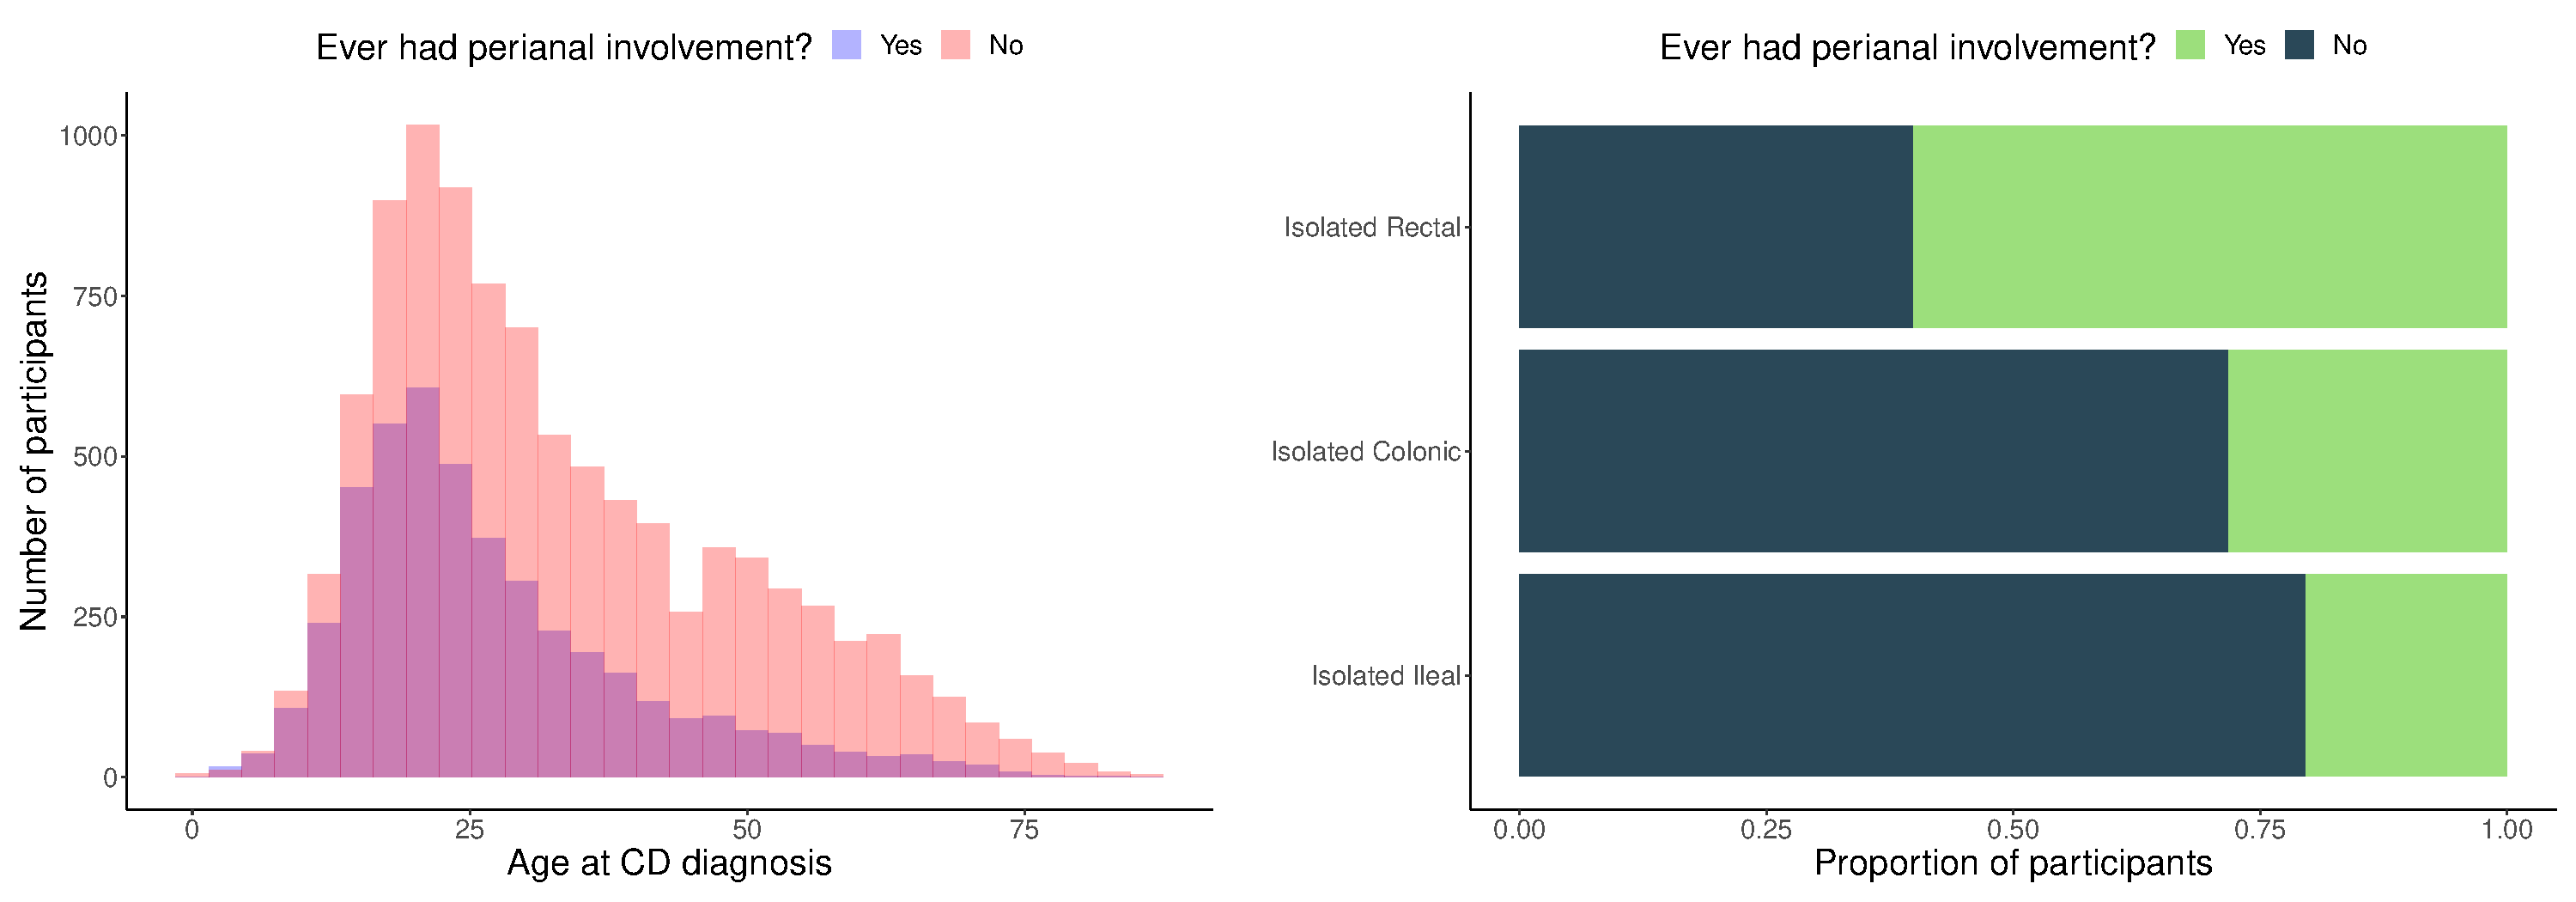
\includegraphics[width=1.0\textwidth]{fig1}
  \caption[Figure]{age at diagnosis and macroscopic extent of Crohn's disease in pCD+ and pCD- patients in the IBD-BR.}
  \label{fig:age_diag_macextent}
  \end{figure}

\subsubsection{Lower rates of drug intake in pCD+ patients in IBD-BR}
pCD+ patients were less likely to be actively prescribed a number of CD medications: oral steroids, Infliximab, Adalimumab, Vedolizumab, and Mesalazine (P-value $<$ 0.0036; Table \ref{table:drug_eim}; odds ratio=0.83, 0.77, 0.62 and 0.55 respectively). Anti-TNF therapies, including Infliximab and Adalimumab, are among the first-line drugs for perianal fistulas, and lead to fistula healing in 50\% of pCD patients (in combination with other surgical procedures) \cite{Regueiro2003-lf,Kotze2014-fh,Haennig2015-pj,Gaertner2007-wb}. Additionally, the ENTERPRISE clinical trial found that Vedolizumab achieved remarkable fistula closure and healing \cite{Schwartz2022-zp}. On the other hand, oral steroids are known to be ineffective for fistula closure and may even exacerbate perianal abscess \cite{Jones1966-tt}. Lower drug intake could therefore be attributed to drug inefficacy, but it could also be a contributing factor to pCD.\\

\subsubsection{pCD+ patients are enriched for six extraintestinal manifestations}
pCD+ patients were enriched for extra-intestinal manifestation compared to pCD- patients (26.3\% versus 19.6\%; P-value $<$ 0.05). Enteropathic arthritis was the most most prevalent extraintestinal manifestation among pCD+ patients, followed by serious infections and psoriasis. In total, six extraintestinal manifestations showed significant enrichment in pCD+ versus pCD- patients (P-value $<$ 0.005; Table  \ref{table:drug_eim}). The association between extraintestinal manifestations was stronger in female participants, possibly since extraintestinal manifestations were more prevalent in female participants overall (odds ratio=1.3 in males versus 1.6 in females). 
\begin{table}
  \centering
  \begin{tabular}[t]{llll}
  \toprule
  \textbf{} & \textbf{pCD+(\%)} & \textbf{pCD-(\%)} & \textbf{P-value}\\
  \midrule
  \addlinespace[0.3em]
  \multicolumn{4}{l}{\textbf{Extraintestinal Manifestations}}\\
  \hspace{1em}Primary Sclerosing Cholangitis & 25 (0.6) & 72 (0.8) & 0.29\\
  \hspace{1em}Enteropathic Arthritis & 413 (9.7) & 635 (6.7) & $2.1\times10^{-9}$\\
  \hspace{1em}Erythema Nodosum & 199 (4.6) & 222 (2.3) & $7.7\times10^{-13}$\\
  \hspace{1em}Iritis & 183 (4.2) & 242 (2.5) & $1.1\times10^{-7}$\\
  \hspace{1em}Orofacial Granulomatosis & 153 (3.6) & 162 (1.7) & $2.4\times10^{-11}$\\
  \hspace{1em}Psoriasis & 311 (7.2) & 518 (5.4) & $6\times10^{-5}$\\
  \hspace{1em}Ankylosing Spndylitis & 110 (2.6) & 238 (2.5) & 0.89\\
  \hspace{1em}Multiple Sclerosis & 9 (0.2) & 27 (0.3) & 0.53\\
  \hspace{1em}Lymphoma & 18 (0.4) & 36 (0.4) & 0.85\\
  \hspace{1em}Serious Infections & 320 (7.4) & 465 (4.9) & $3.2\times10^{-9}$\\
  \addlinespace[0.3em]
  \multicolumn{4}{l}{\textbf{Drugs}}\\
  \hspace{1em}Azathioprine & 1373 (41.4) & 2649 (42.1) & 0.49\\
  \hspace{1em}Mercaptopurine & 271 (35.6) & 564 (36.1) & 0.83\\
  \hspace{1em}Methotrexate & 192 (28.6) & 404 (35.4) & ${4\times10^{-3}}$\\
  \hspace{1em}Infliximab & 1207 (50.9) & 1622 (55.7) & $6\times10^{-4}$\\
  \hspace{1em}Adalimumab & 740 (47.8) & 1368 (54.2) & $8\times10^{5}$\\
  \hspace{1em}Vedolimumab & 236 (67.8) & 424 (77.4) & $2\times10^{-3}$\\
  \hspace{1em}Ustekinumab & 171 (69.2) & 209 (72.6) & 0.45\\
  \hspace{1em}Mesalazine & 528 (30) & 1649 (43.7) & $< 2.2\times10^{-16}$\\
  \hspace{1em}Oral Steroids & 304 (11.3) & 823 (14.2) & $3\times10^{-4}$\\
 
  \bottomrule
  \end{tabular}
  \caption{Drug intake and extraintestinal manifestations in pCD+ and pCD- patients in the IBD-BR. Percentage of patients are shown between parentheses. Significant differences between pCD+ and pCD- were assesed using a $\chi^{2}$ test and the P-value is shown in the last column.}
  \label{table:drug_eim}
  \end{table}
  
% \begin{table}[htbp!]
%   \centering
%   \begin{tabular}{|l|l|l|r|}
%   \hline
%   Drug          & pCD+        & pCD-        & \multicolumn{1}{l|}{P-value} \\ \hline
%   Aza           & 1373 (41.4) & 2649 (42.1) & 0.4932629                    \\ \hline
%   Merc          & 271 (35.6)  & 564 (36.1)  & 0.8335190                    \\ \hline
%   Metho         & 192 (28.6)  & 404 (35.4)  & 0.0036395                    \\ \hline
%   Inflix        & 1207 (50.9) & 1622 (55.7) & 0.0006321                    \\ \hline
%   Ada           & 740 (47.8)  & 1368 (54.2) & 0.0000796                    \\ \hline
%   Goli          & 9 (56.2)    & 9 (50)      & 0.9838468                    \\ \hline
%   Vedo          & 236 (67.8)  & 424 (77.4)  & 0.0020198                    \\ \hline
%   Ust           & 171 (69.2)  & 209 (72.6)  & 0.4514008                    \\ \hline
%   Mesa          & 528 (30)    & 1649 (43.7) & 0.0000000                    \\ \hline
%   Oral\_ster    & 304 (11.3)  & 823 (14.2)  & 0.0002656                    \\ \hline
%   Other1\_treat & 195 (37.9)  & 434 (49.6)  & 0.0000318                    \\ \hline
%   Extraintestinal manifestations & pCD+      & pCD-      & \multicolumn{1}{l|}{P-value} \\ \hline
%   prim\_scler\_chol              & 25 (0.6)  & 72 (0.8)  & 0.2916513                    \\ \hline
%   enter\_arth                    & 413 (9.7) & 635 (6.7) & 0.0000000                    \\ \hline
%   ery\_nodo                      & 199 (4.6) & 222 (2.3) & 0.0000000                    \\ \hline
%   iritis                         & 183 (4.2) & 242 (2.5) & 0.0000001                    \\ \hline
%   oro\_gran                      & 153 (3.6) & 162 (1.7) & 0.0000000                    \\ \hline
%   psori                          & 311 (7.2) & 518 (5.4) & 0.0000596                    \\ \hline
%   ank\_spond                     & 110 (2.6) & 238 (2.5) & 0.8860326                    \\ \hline
%   mult\_scler                    & 9 (0.2)   & 27 (0.3)  & 0.5346415                    \\ \hline
%   lymphoma                       & 18 (0.4)  & 36 (0.4)  & 0.8479312                    \\ \hline
%   ser\_infect                    & 320 (7.4) & 465 (4.9) & 0.0000000                    \\ \hline
%   \end{tabular}
%   \end{table}
  % \begin{table}[]
  %   \centering
  %   \begin{tabular}{|l|l|l|r|}
  %   \hline
  %   Extraintestinal manifestations & pCD+      & pCD-      & \multicolumn{1}{l|}{P-value} \\ \hline
  %   prim\_scler\_chol              & 25 (0.6)  & 72 (0.8)  & 0.2916513                    \\ \hline
  %   enter\_arth                    & 413 (9.7) & 635 (6.7) & 0.0000000                    \\ \hline
  %   ery\_nodo                      & 199 (4.6) & 222 (2.3) & 0.0000000                    \\ \hline
  %   iritis                         & 183 (4.2) & 242 (2.5) & 0.0000001                    \\ \hline
  %   oro\_gran                      & 153 (3.6) & 162 (1.7) & 0.0000000                    \\ \hline
  %   psori                          & 311 (7.2) & 518 (5.4) & 0.0000596                    \\ \hline
  %   ank\_spond                     & 110 (2.6) & 238 (2.5) & 0.8860326                    \\ \hline
  %   mult\_scler                    & 9 (0.2)   & 27 (0.3)  & 0.5346415                    \\ \hline
  %   lymphoma                       & 18 (0.4)  & 36 (0.4)  & 0.8479312                    \\ \hline
  %   ser\_infect                    & 320 (7.4) & 465 (4.9) & 0.0000000                    \\ \hline
  %   \end{tabular}
  %   \end{table}

% \subsubsection{pCD and extraintestinal manifestations: other factors to consider}
% Other factors that may underlie this enrichment include treatment with anti-TNFs such as Infliximab, which are effective in reducing extraintestinal manifestations. In the previous section, I showed that pCD+ patients in IBD-BR are less likely to be actively taking a number of drugs including Infliximab. Therefore, an important question is whether this enrichment is driven by true shared pathophysiology between pCD and extraintestinal manifestations, or if it is merely due to lower rates of Infliximab intake in pCD+ patients (as well as other drugs).\\

% This can be tested by assessing the enrichment of extraintestinal manifestations within subsets of patients stratified by drug intake (e.g. patients currently on Infliximab versus patients not on Infliximab). If stratifying by drug intake does not affect the enrichment, then t is unlikely to be driven by drug intake. 
% However, information on drug intake, pCD and extraintestinal manifestations were jointly available for a smaller set of IBD-BR participants (n=5,133-5,186) that did not exhibit an enrichment of extraintestinal manifestations in pCD+ versus pCD- patients. Therefore, these sets of participants cannot be used to make a conclusion about the effect of drug intake on the observed enrichment in participants with pCD information. 




    \subsubsection{Surgical burden of pCD}

    Combined surgical and medical interventions represent some of the few effective interventions available to pCD patients. Different surgical options are available to perianal disease patients depending on its anatomical features, complications and disease severity. Exploration under anaesthesia and seton insertion are the typical first-line management options, and further medical or surgical interventions are based on initial exploration \cite{Adegbola2018-ha}. As expected, 2,971 pCD patients (66.8\%) had undergone any type of surgical intervention compared to 3,637 (37.2\%) of pCD- participants. In total, almost half the pCD+ patients with operative history had undergone one of three pCD-related surgical procedures (1431 patients; 48.2\%): drainge of perianal abscess, insertion of seton, or drainage of fistula. Perianal abscess drainage was the most common: 808 pCD+ patients (27.2\% of surgically-operated patients) underwent at least one perianal abscess drainage operation, followed by insertion of a seton suture (744 pCD+ patients; 25\%), followed by perianal fistula repair operation (438 pCD+ patients; 14.7\%).

    \subsubsection{pCD prevalence decreased over time}
    Understanding pCD prevalence over time is important to understand how the burden of pCD on patients and healthcare providers has changed. Previous work has shown reduced pCD incidence over the last decade \cite{Park2019-kj}, which was partly attributed to improved treatment options. In this regard, IBD-BR offers a unique opportunity to assess this trend. Although the precise time of pCD development is not avaialble, the time between CD diagnosis and the last clinical review can be used to compare how pCD prevalence among CD patients has changed in different eras. Over 93\% of IBD-BR patients with pCD information were clinically re-assessed in or later than 2016, which reduces the bias introduced by potentially outdated clinical data. \\
    
    To investigate this trend in the IBD-BR, I partitioned participants according to their year of CD diagnosis into two-year groups (e.g. 2006-2008), and calculated prevalence estimates in each period. As expected, confidence intervals around the point estimates were larger in the years between 1980-2010 since fewer IBD-BR patients were diagnosed with CD in those years (100-230 participants per two years). This rose to 497-734 per two years in the years from 2010 to 2020.  Notably, point prevalence estimates decreased starting from the year 2010 onwards. The mean point prevalence between 1980 to 2010 decreased significantly from 35.9\% to 25.1\% between 2010 to 2020 (t-test P-value $<2\times10^{-16}$; Figure \ref{fig:pcd_prev}). The decrease in prevalence remained significant when mean point prevalence was calculated between 2010 to 2016 only (mean prevalence=26.8\%), between 2010 to 2014 only (mean prevalence=28.1\%), or between 2010 to 2012 (mean prevalence=29.4\%).\\
    \begin{figure}[htb] 
      \centering    
      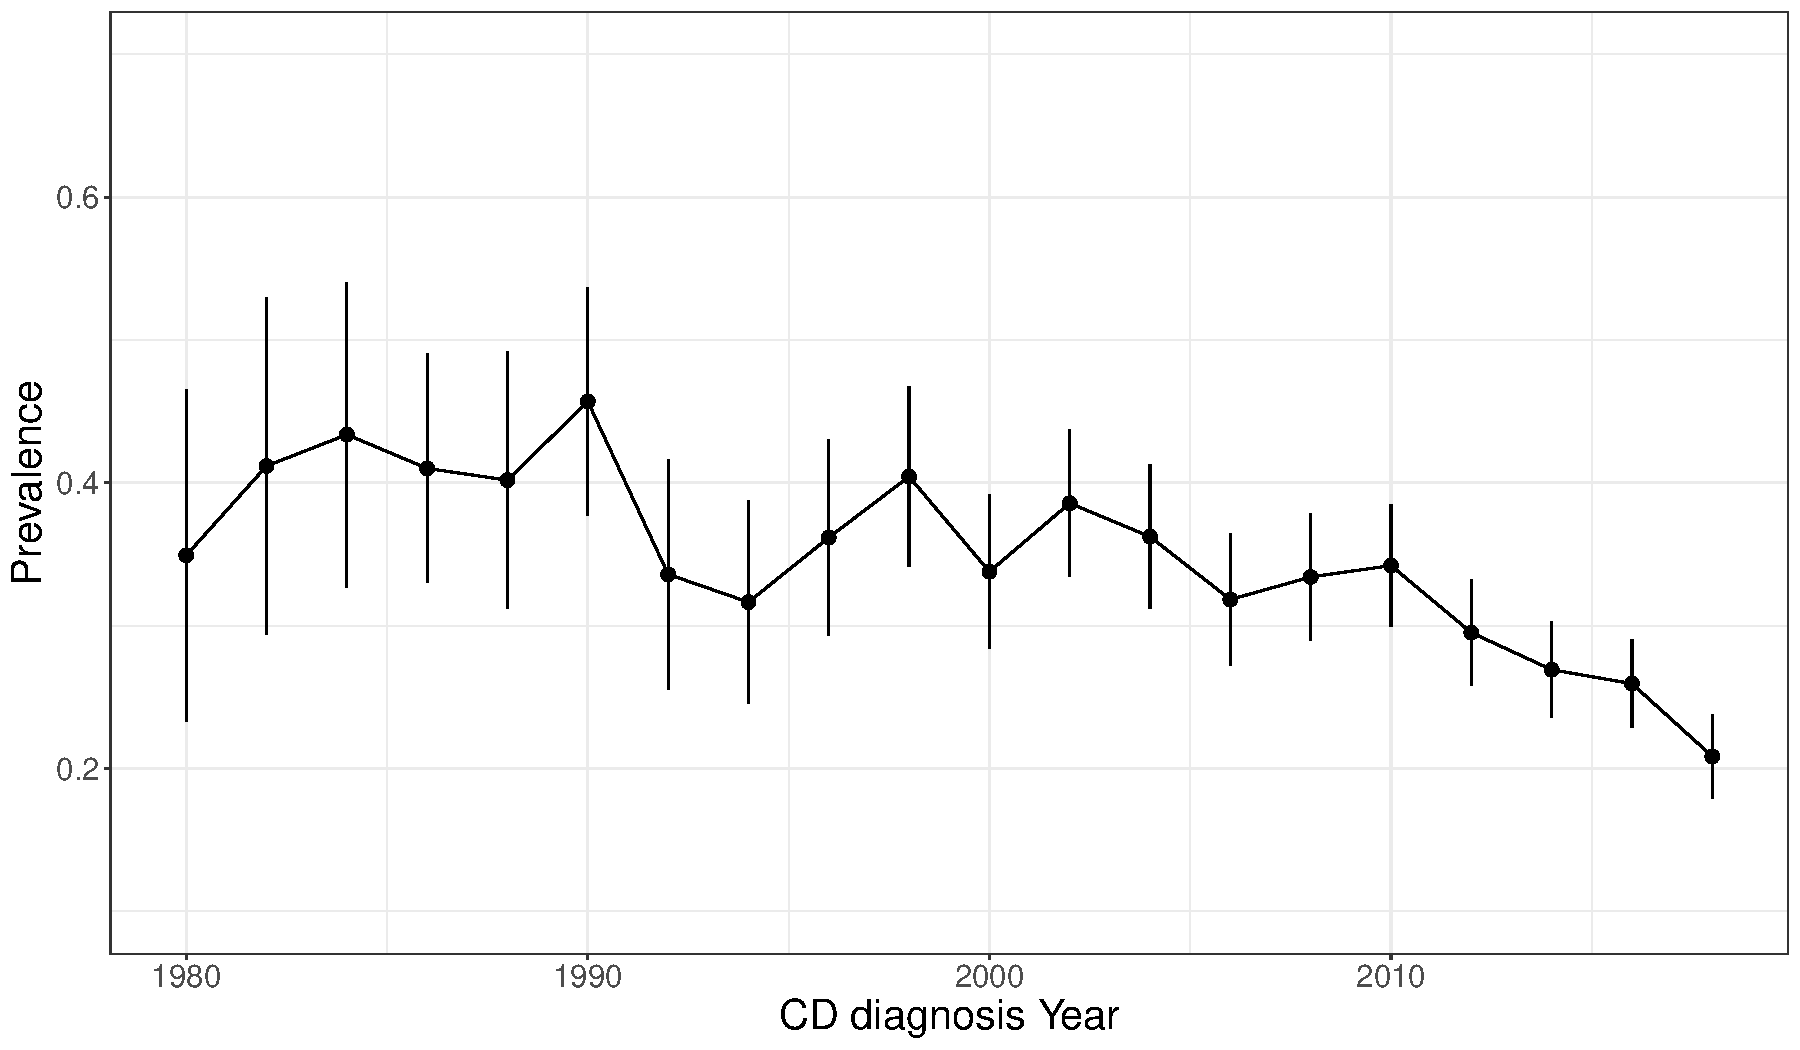
\includegraphics[width=1.0\textwidth]{fig2}
      \caption[Figure]{Prevalence per year of CD diagnosis, partitioned into two-year groups. 95\% confidence intervals around point estimates are calculated using a bootstrap procedure, whereby participants where resampled 1,000 times within each two-year group.}
      \label{fig:pcd_prev}
      \end{figure}
 
    A decrease in pCD prevalence has been observed previously \cite{Park2019-kj}. However, such a decrease has not been precisely quantified, partly due to the relatively smaller sample sizes of most studies \cite{Brochard2022-kz,Bruckner2018-ag,Gottgens2017-df,Tsai2022-kz}. A potential limitation of this analysis is that censored data may contribute to the observed decrease in pCD prevalence in later years. pCD does not always present at the time of diagnosis, which may bias prevalence estimates downwards in the years after 2010. An important consideration when investigating the effect of data censorship is that pCD prevalence estimates should be up-to-date. For example, a patient who is diagnosed with CD in 2012 for example may be incorrectly considered pCD-free if their clinical information were not updated afterwards. In IBD-BR, this bias is mitigated by the the fact that the majority of patients were clinically assessed between 2016 and 2021. Additionally, the consistent decrease in pCD prevalence even when I excluded patients diagnosed after 2016, 2014, or 2012 indicates that the contribution of censored observation is likely minimal. Although some patients may develop perianal symptoms up to 20 years after diagnosis, the cumulative probability of developing pCD does not increase significantly after 5 years \cite{Tsai2022-kz}. It is therefore unlikely that the decrease in pCD prevalence is affected by censored observations.

    \subsection{UKIBDGC and IBD-BR definitions of pCD are similar}
    Similar to IBD-BR, the UKIBDGC can be used to define a pCD+/pCD- cohort. The UKIBDGC reports a number of clinical and phenotypic characteristics of IBD patients. For each IBD participant, disease subtype diagnosis, and location (inclduding perianal disease) are recorded. However, it is unclear whether the criteria for assigning pCD status is consistent between the different centers, and more importantly if it matches the criteria used to assign pCD status to IBD-BR patients. Heterogeneity in pCD status definition can often arise from different diagnostic criteria being applied, or different times of phenotype update between patients. Ensuring the consistency of pCD status between UKIBDGC and IBD-BR is crucial to minimise the heterogeneity of phenotype definition between the two cohorts and maximise the statistical power from a meta-analysis between the two cohorts. 
To assess this, participants who may have taken part in both the IBD-BR and UKIBDGC can be leveraged to understand the level of agreement in pCD status assignment. Since participant identifiers are not mapped across studies, genetic similarity of individuals across cohorts can instead be leveraged to identify overlapping participants (Methods).\\

Out of 971 overlapping CD participants, only one participant exhibited discordant pCD status between IBD-BR and UKIBDGC. A total of 432 participants had missing or “Unknown” perianal involvement, 406 of which were“Unknown” in both cohorts (Table \ref{table:cohort_pcd_agree}). This strong agreement in pCD status indicates that both cohorts assign pCD status in a similar fashion.\\

I then asked if the UKIBDGC cohort was enriched for particular perianal manifestations. Since this information is not available in the UKIBDGC phenotype data, it can be obtained from the IBD-BR clinical data for patients who reported pCD+ status in both studies. I found that these patients were not enriched in any particular type of perianal involvement (e.g. 51.9\% of overlapping individuals reported either simple or complex fistula versus 52\% in IBD-BR). Moreover, 27\% of the overlapping patients reported only skin tags, fissures or ulcer, indicating that milder forms of pCD were also included in the UKIBDGC assignment of pCD+ status. Overall, this shows that the definition of pCD status is likely consistent between the cohorts. From the analysis of overlapping individuals it does not appear that the UKIBDGC pCD status assignment criteria were different from the criteria used in the IBD-BR questionnaire.


\begin{table}[htb]
  \caption{Number of overlapping individuals between UKIBDGC and IBD-BR who answered Yes, No or Unknown to \textit{Ever had perianal involvement?}}
  \label{table:cohort_pcd_agree}
  \centering
  \begin{tabular}[t]{|l|r|r|r|}
  \hline
  \multicolumn{1}{|c|}{ } & \multicolumn{3}{c|}{UKIBDGC} \\
  \cline{2-4}
  IBD-BR& Yes & No & Unknown\\
  \hline
  Yes & 201 & 0 & 1\\
  \hline
  No & 1 & 337 & 6\\
  \hline
  Unknown & 6 & 13 & 406\\
  \hline
  \end{tabular}
  \end{table}

  \section{Genome-wide association analysis of pCD}
  \subsection{Defining pCD+ cases}
  Genome-wide studies of disease subphenotypes pose unique challenges compared to traditional case-control GWASes. Unlike GWASes of CD, for example, where robust diagnostic criteria are applied to clearly demarcate cases and controls, in GWAS of disease subphenotype such as pCD it is not obvious which specific manifestations should be considered cases. The IBD-BR questionnaire reports several types of pCD manifestations, including skin tags, fissures or ulcers, perianal abscess, and simple and complex fistulas. In this chapter, my aim is to perform a pCD meta-analysis between IBD-BR and UKIBDGC, and therefore similarity in pCD+ case definition across the cohorts is an important consideration to ensure the robustness of genome-wide significant hits. In the previous section, I showed that leveraging individuals who registered for both studies can give an insight into the composition of the UKIBDGC pCD+ cases. This showed that UKIBDGC pCD+ cases were not particularly enriched in any particular type of perianal manifestations. Additionally, when I inspected the UKIBDGC questionnaire used to collect perianal manifestations data, I found that the relevant question appeared to include all types of perianal manifestations: \textit{"Ever had perianal fistula (incl recto-vaginal),  abscess, anal ulcer or significant anal stenosis?"}. I threfore defined pCD+ cases in both cohorts as CD patients that report any type of perianal involvement,
  
 
\subsection{IBD-BR}
Although clinical and phenotypic data are available for all participants, not all participants have been genotyped in the current release (04/04/2022). From a total of 15,152 participants with CD diagnosis, 9,458 European ancestry participants with perianal involvement data were genotyped. To ensure that pCD- controls do not include recently diagnosed CD patients who may develop perianal disease in the near future, I excluded pCD- controls diagnosed with CD less than 5 years before the last clinical review. This choice was informed by previous studies that showed that the cumulative risk of developing perianal disease 5 years and 10 years after diagnosis are similar \cite{Tsai2022-kz}. This resulted in a total of 6833 participants (2,664 pCD+ cases and 4,169 pCD- controls). After these filters were applied, the composition of genotyped pCD+ cases cohort matched the overall composition of all participants with perianal involvement information reported earlier. 53.6\% (1480) of genotyped pCD+ individuals had either a simple or complex perianal fistula, and 41.2\% (1098) had perianal abscess. Together, patients with perianal fistula or abscess account for 74.9\% (1995) of genotyped pCD+ cases.\\

With the pCD case-control cohort defined above, I performed GWAS between pCD+ cases and pCD- controls using REGENIE and used four European-ancestry genotypic principal components and sex as covariates. I removed variants with imputation INFO score < 0.4 and minor allele frequency (MAF) < 0.01, leaving 9,777,139 variants for association analysis (see Methods for detailed genotype and imputation QC). None of the tested variants achieved genome-wide significant association (P-value $< 5\times10^{-8}$). There was moderate evidence of genomic inflation (median $\chi^{2}$=0.49; $\lambda_{GC}$=1.08).
\subsection{UKIBDGC}
As mentioned earlier, UKIBDGC only reports whether or not partipcipants report perianal involvement and does not provide specific perianal manifestations. A total of 8,078 patients of European ancestry were diagnosed with CD, of which 6550 had perianal involvement information. To minimise sample overlap with the IBD-BR, I removed UKIBDGC individuals who showed genetic similarity with individuals from the IBD-BR (see Methods for more details on how genetic similarity was assessed), and performed GWAS with the remaining individuals (1303 pCD+ and 4761 pCD-). \\

I performed GWAS similar to the IBD-BR analysis, with the difference that UKIBDGC samples were genotyped with two different gentopying arrays and were therefore analysed seperately (I will refer to these two cohorts as HCE and GWAS1; Methods). A total of 8,916,200 and 8,897,554 variants were tested in HCE and GWAS1, respectively. No variants achieved genome-wide significant association (P-value < $5\times10^{-8}$). There was no evidence of genomic inflation (HCE: median $\chi^{2}$=0.47; $\lambda_{GC}$=1.04; GWAS1: median $\chi^{2}$=0.46; $\lambda_{GC}$=1.01).

\subsection{Meta-analysis between UKIBGC and IBD-BR: a genome-wide significant locus at 6p21.32}

I used METAL to perform a fixed-effects meta-analysis between summary statistics from IBD-BR, and the two UKIBDGC summary statistics HCE and GWAS1, with a total of 3,967 pCD+ cases and 8,930 pCD- controls. 
  Four variants in the MHC region at the 6p21.32 locus showed genome-wide significant association (index variant rs115378818; P-value=$8.6\times10^{-12}$; Table \ref{table:gws}). None of the variants showed significant heterogeneity of effect size between the constituent cohorts ($P_{het}$ < 0.008). All four variants were well-imputed across the constituent cohorts (INFO score > 0.7).
  \begin{table}[H]
    \caption{Genome-wide significant variants in the 6p21.32 locus. Odds ratio and their 95\% confidence intervals are shown. MAF=minor allele frequency.}
    \label{table:gws}
    \centering\begingroup\fontsize{10}{12}\selectfont
    
    \begin{tabular}[t]{|r|l|l|l|l|l|}
    \hline
    Chromosome & Position (b38) & Effect Allele & OR & P-value & MAF\\
    \hline
    6 & 32,205,822 & C & 1.45 (1.27 - 1.66) & $4\times10^{-8}$ & 0.05\\
    \hline
    6 & 32,243,461 & C & 1.38 (1.23 - 1.55) & $4.4\times10^{-8}$ & 0.08\\
    \hline
    6 & 32,279,268 & G & 1.57 (1.36 - 1.82) & $1.5\times10^{-9}$ & 0.05\\
    \hline
    6 & 32,333,650 & T & 1.78 (1.51 - 2.1) & $8.6\times10^{-12}$ & 0.04\\
    \hline
    \end{tabular}
    \endgroup{}
    \end{table}

    \begin{table}[H]

      \caption{\label{tab:table:maf_concord_cc}Case and control minor allele frequencies of the genome-wide significant variants in the 6p21.32 locus in all constituent cohorts.}
      \centering
      \fontsize{9}{11}\selectfont
      \begin{tabular}[t]{>{\raggedright\arraybackslash}p{5em}>{\raggedleft\arraybackslash}p{3em}>{\raggedleft\arraybackslash}p{3em}>{\raggedleft\arraybackslash}p{3em}>{\raggedleft\arraybackslash}p{3em}>{\raggedleft\arraybackslash}p{3em}>{\raggedleft\arraybackslash}p{3em}}
      \toprule
      \multicolumn{1}{c}{ } & \multicolumn{2}{c}{IBD-BR} & \multicolumn{2}{c}{UKIBDGC (HCE)} & \multicolumn{2}{c}{UKIBDGC (GWAS1)} \\
      \cmidrule(l{3pt}r{3pt}){2-3} \cmidrule(l{3pt}r{3pt}){4-5} \cmidrule(l{3pt}r{3pt}){6-7}
      SNP & Cases & Controls & Cases & Controls & Cases & Controls\\
      \midrule
      6:32333650\_C\_T & 0.042 & 0.027 & 0.059 & 0.037 & 0.055 & 0.035\\
      6:32279268\_T\_G & 0.054 & 0.038 & 0.067 & 0.046 & 0.062 & 0.044\\
      6:32205822\_T\_C & 0.063 & 0.046 & 0.070 & 0.051 & 0.065 & 0.047\\
      6:32243461\_G\_C & 0.084 & 0.066 & 0.092 & 0.073 & 0.099 & 0.072\\
      \bottomrule
      \end{tabular}
      \end{table}
%%%%%%%%%%%%%%%%%%%%%%%%%%%%%%%%%%%%%%%%%
%FIGURE SOURCE: /nfs/users/nfs_o/oe2/ibdbr/scripts/explore/manhattan.R
%%%%%%%%%%%%%%%%%%%%%%%%%%%%%%%%%%%%%%%%%

All four variants had a low minor allele frequency (MAF), ranging from  0.04 to 0.08 in the constituent cohorts (Table \ref{table:gws}). Low-frequency variant calling is more prone to genotyping errors than common variants, and therefore low-frequency genome-wide significant hits require additional quality checks. In some studies, these associations were later found to be false positives \cite{Tabangin2009-gs,Ayers2011-bc}. To minimise this risk and ensure the robustness of the associated variants, I performed a post-GWAS to investigate whether the association evidence is consistent with the expected LD structure between variants in non-Finnish Europeans. This check ensures that variants in the genome-wide significant locus follow their expected LD. Mismatches between association strength and expected LD reflects a potential false positive association.\\
\begin{figure}[H]
  \centering   
  \begin{subfigure}[t]{1.0\textwidth}
    \centering   

    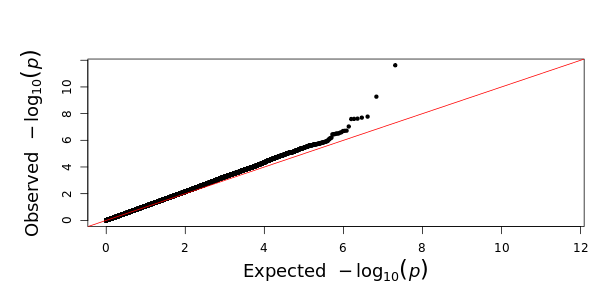
\includegraphics[width=1.0\textwidth]{Vector/ukibdgc_ibdbr_perianal_timesincediag5yrsctrl_allcase_meta_qq}

    
  \end{subfigure} 

    \begin{subfigure}[t]{1.0\textwidth}
      \centering   

      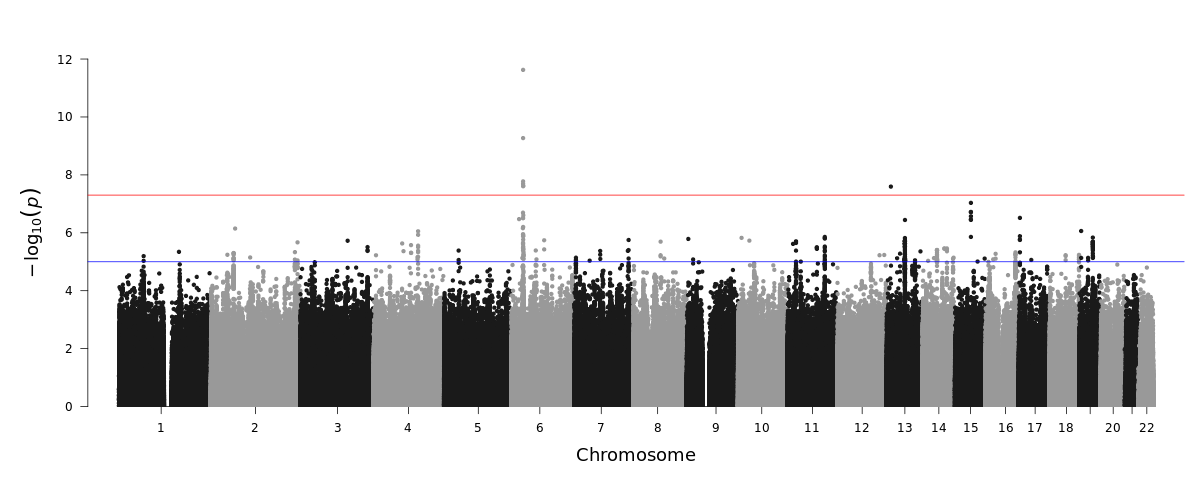
\includegraphics[width=0.8\textwidth]{Vector/ukibdgc_ibdbr_perianal_timesincediag5yrsctrl_allcase_meta}

      
  \end{subfigure} 
  \caption[Figure]{(a) Quantile-quantile plot for the meta-analysis between UKIBDGC and IBD-BR cohorts, suggesting a good fit to the uniform distribution, and showing no evidence of genomic inflation (median $\chi^{2}$=0.47; $\lambda_{GC}$=1.03; median $\chi^{2}$ was calculated by converting P-values to $\chi^{2}$  values using the function \Verb+qchisq(P, df=1,lower.tail=F)+ in R v4.1.0). (b) Manhattan plot of meta-analysis between IBD-BR and UKIBDGC. pCD+ cases are defined as CD patients with any type of perianal involvement and pCD- controls are defined as CD patients with no perianal involvement.}
  \label{fig:meta_qq_manhattan}
  \end{figure}
  % \begin{figure}[H] 
  %   \centering    
  %   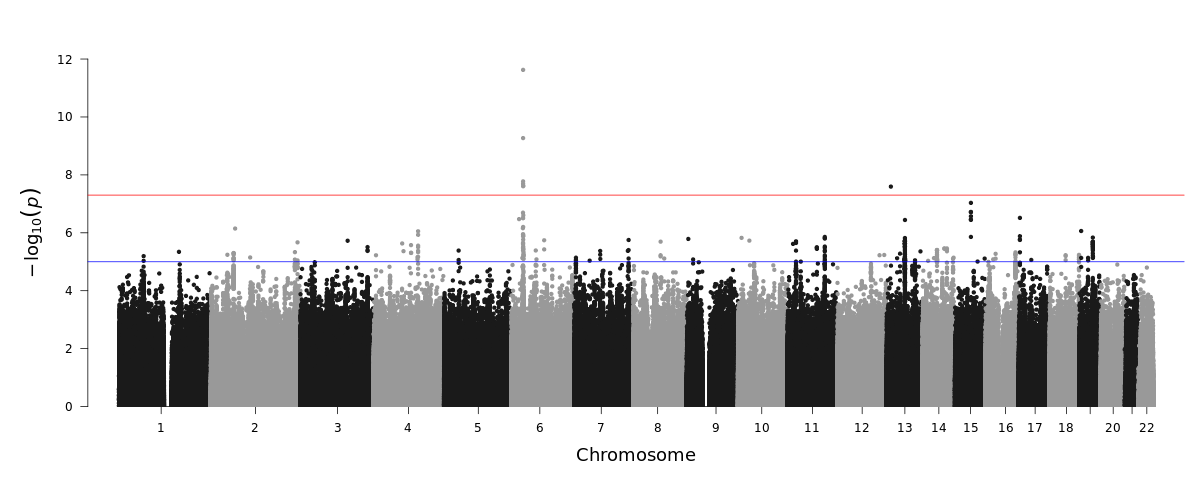
\includegraphics[width=1.0\textwidth]{Vector/ukibdgc_ibdbr_perianal_timesincediag5yrsctrl_allcase_meta}
  %   \caption[Figure]{Manhattan plot of meta-analysis between IBD-BR and UKIBDGC. pCD+ cases are defined as CD patients with any type of perianal involvement and pCD- controls are defined as CD patients with no perianal involvement.}
  %   \label{fig:meta_manhattan}
  %   \end{figure}

  


  % \subsubsection{Power analysis}
  % The ability of a GWAS study to make genome-wide significant discoveries depends on its statistical power. Statistical power is defined as the probability of correctly declaring genome-wide significance, when the alternative hypothesis that a variant is genome-wide significant it true. Statistical power analysis can therefore be used as a diagnostic test to check if the discovered variants are expected under a given study sample size its case proportion. Given a variant's MAF, effect size, a power value close to 1 indicates that the discovery is indeed expected given the study sample size. Generally, I found that the study was adequately powered to discover three of the four genome-wide significant variants (power > 0.8), and one of the variants was detectable with a power of 0.78 (Figure \ref{fig:power_analysis}). The study had an almost complete power to detect 6:32279268\_T\_G and 6:32333650\_C\_T, the two most significant variants (power > 0.98). This shows that the meta-analysis is reasonably powered to detect the genome-wide significant locus. 

  %   \begin{figure}[H] 
  %     \centering    
  %     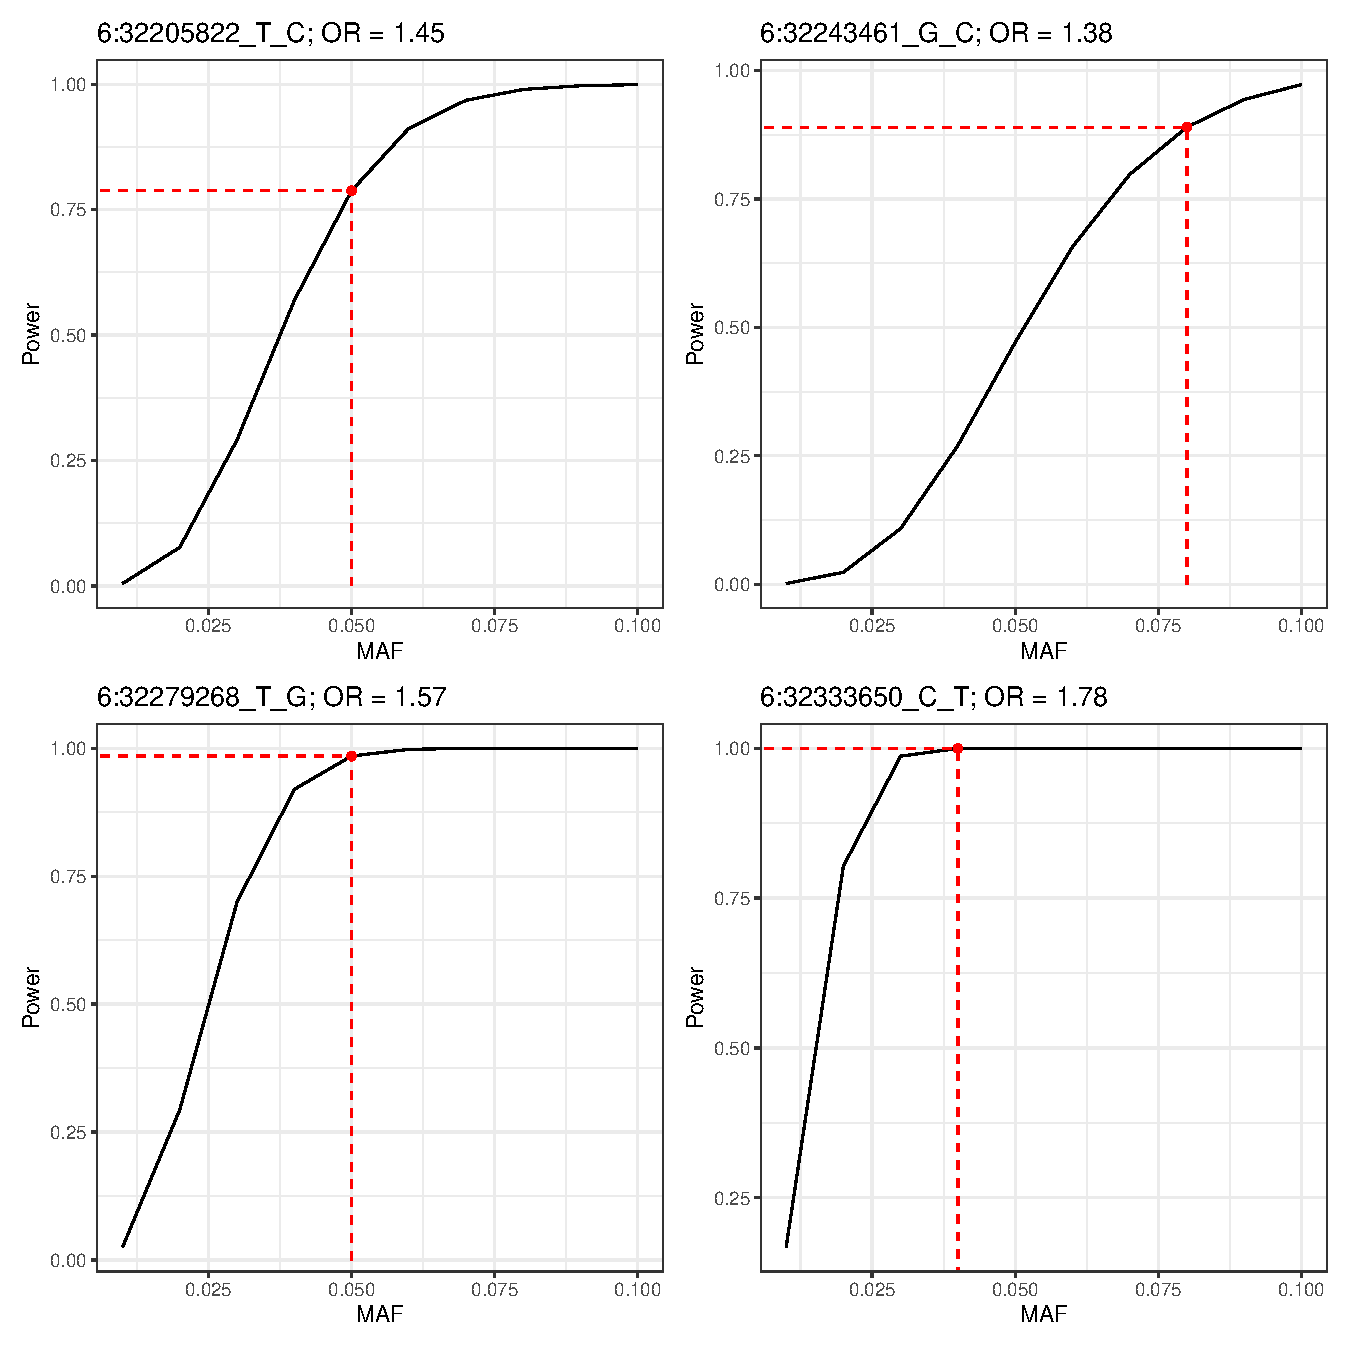
\includegraphics[width=0.7\textwidth]{power_analysis}
  %     \caption[Figure]{Power analysis for each of the genome-wide significant variants over a range of MAFs. Title, red dots and dotted lines indicate the MAF and power of the variant}
  %     \label{fig:power_analysis}
  %     \end{figure}
    
     
    \begin{figure}[H] 
      \centering    
      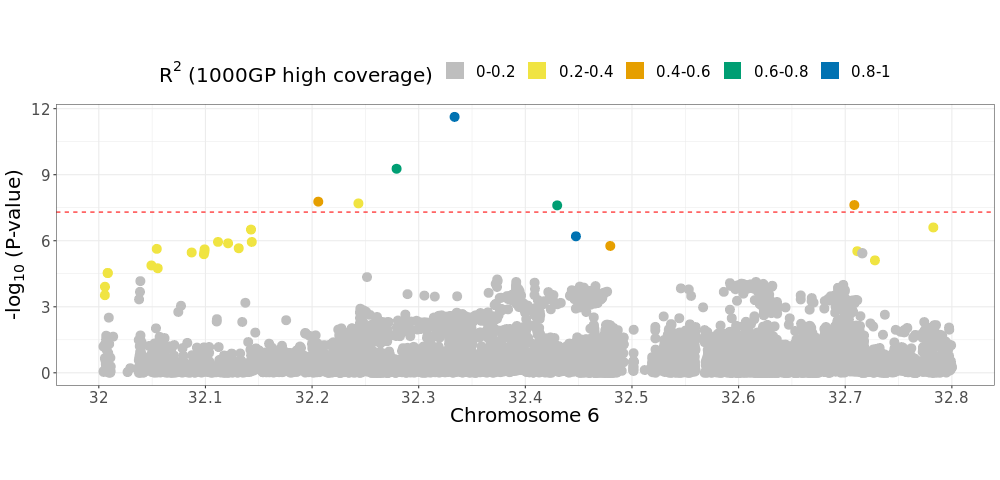
\includegraphics[width=0.8\textwidth]{Vector/regional_assoc_plot}
      \caption[Figure]{Regional association plot showing meta-analysis association P-values in 6p21.32. Variants are coloured by $R^{2}$ with the index variant, derived from 1000 Genomes Project High Coverage study (Non-Finnish Europeans)}
      \label{fig:regional_assoc_plot}
      \end{figure}
%     \subsubsection{Consistency of MAFs at 6p21.32}
   
%   The meta-analysis combined summary statistics from two different IBD cohorts genotyped using three arrays and three imputation reference panels. Given this multitude of genotyping and imputation platforms, it is conceivable that poor genotyping and/or imputation could lead to unreliable results in one of the cohorts. Additionally, cryptic population structure that is specific to one of the cohorts could also contribute to spurious associations. Checking the consistency of MAF across the cohorts can give an assurance that the genome-wide significant associations at this locus are reliable. 
  
  
%  First, I observed that all variants had consistently higher cohort than population MAFs (Table \ref{tab:table:maf_concord}). Such a systematic difference in MAF may be expected if these variants are also associated with CD risk, since the constituent cohorts are composed entirely of CD patients. In support of this, I found that two of the four variants were associated with CD in an independent UKBB-based GWAS study, explaining the higher cohort MAFs (replication P-value < 0.025).  Moreover, I compared case and control MAFs across cohorts, and found that case MAFs were systematically higher than control MAFs, which is expected given the pCD-risk-increaseing effect of the minor alleles. More importantly, case MAFs were consistent across cohorts, as were control MAFs (index variant case MAF: 0.042, 0.059, and 0.055; control MAF: 0.027, 0.037, and 0.035, in IBD-BR, UKIBGC-HCE and UKIBDGC-GWAS1 respectively).

%     \begin{table}[H]

%       \caption{\label{tab:table:maf_concord}Minor allele frequencies for the genome-wide significant variants in the 6p21.32 locus in the meta-analysis constituent cohorts, and in two population cohorts (1000 Genomes Project and GnomAD; Non-Finnish Europeans). Association P-value with Crohn's Disease are shown (obtained from the Open Targets Genetics Portal).}
%       \centering
%       \fontsize{9}{11}\selectfont
%       \begin{tabular}[t]{lrrrrrl}
%       \toprule
%       \multicolumn{1}{c}{ } & \multicolumn{2}{c}{Population Cohorts} & \multicolumn{3}{c}{Study Cohorts} & \multicolumn{1}{c}{ } \\
%       \cmidrule(l{3pt}r{3pt}){2-3} \cmidrule(l{3pt}r{3pt}){4-6}
%       SNP & 1000GP & GnomAD & IBD-BR & UKIBDGC (HCE) & UKIBDGC (GWAS1) & CD P-value\\
%       \midrule
%       6:32333650\_C\_T & 0.012 & 0.012 & 0.033 & 0.041 & 0.042 & NA\\
%       6:32279268\_T\_G & 0.015 & 0.020 & 0.044 & 0.050 & 0.050 & NA\\
%       6:32205822\_T\_C & 0.021 & 0.028 & 0.053 & 0.054 & 0.053 & $4.8\times10^{-11}$\\
%       6:32243461\_G\_C & 0.036 & 0.052 & 0.074 & 0.076 & 0.081 & $5.6\times10^{-7}$\\
%       \bottomrule
%       \end{tabular}
%       \end{table}
  

    \subsubsection{Association signal at 6p21.32 matches expected linkage disequilibrium pattern in non-Finnish Europeans}
    Although the four variants spanned a 130 kbp region, they displayed high LD with the index variant, as the 6p21 region is known to exhibit long-range LD (Figure \ref{fig:regional_assoc_plot}). To better understand if the association strength matches the expected LD pattern, I measured the correlation between the association P-value and $R^{2}$ with the index variant. The underlying assumption is that, for a given variant in a locus, the lower its LD with the index variant, the weaker its association is expected to be. P-values that do not match this expectation may suggest a spurious association due to a genotyping or imputation error or cryptic population structure. At 6p21.32, I found that LD friends P-values were correlated with the expected $R^{2}$ with the index variant ($\rho$=0.45; LD friends defined as variants with $R^{2}$ > 0.5 with the index variant and P-value < 0.01; Figure \ref{fig:ld_pval_plot}). The relatively weak correlation is likely driven by the small number of LD friends that the index variant has (N=4). When I relaxed the $R^{2}$ cutoff of LD friends this correlation became increasingly stronger ($\rho$=0.65 and 0.72 at $R^{2}$ > 0.4 and 0.2, respectively), showing that overall the variants at this locus follow their expected association strength given the LD structure between variants. 




    \begin{figure}[H] 
      \centering    
      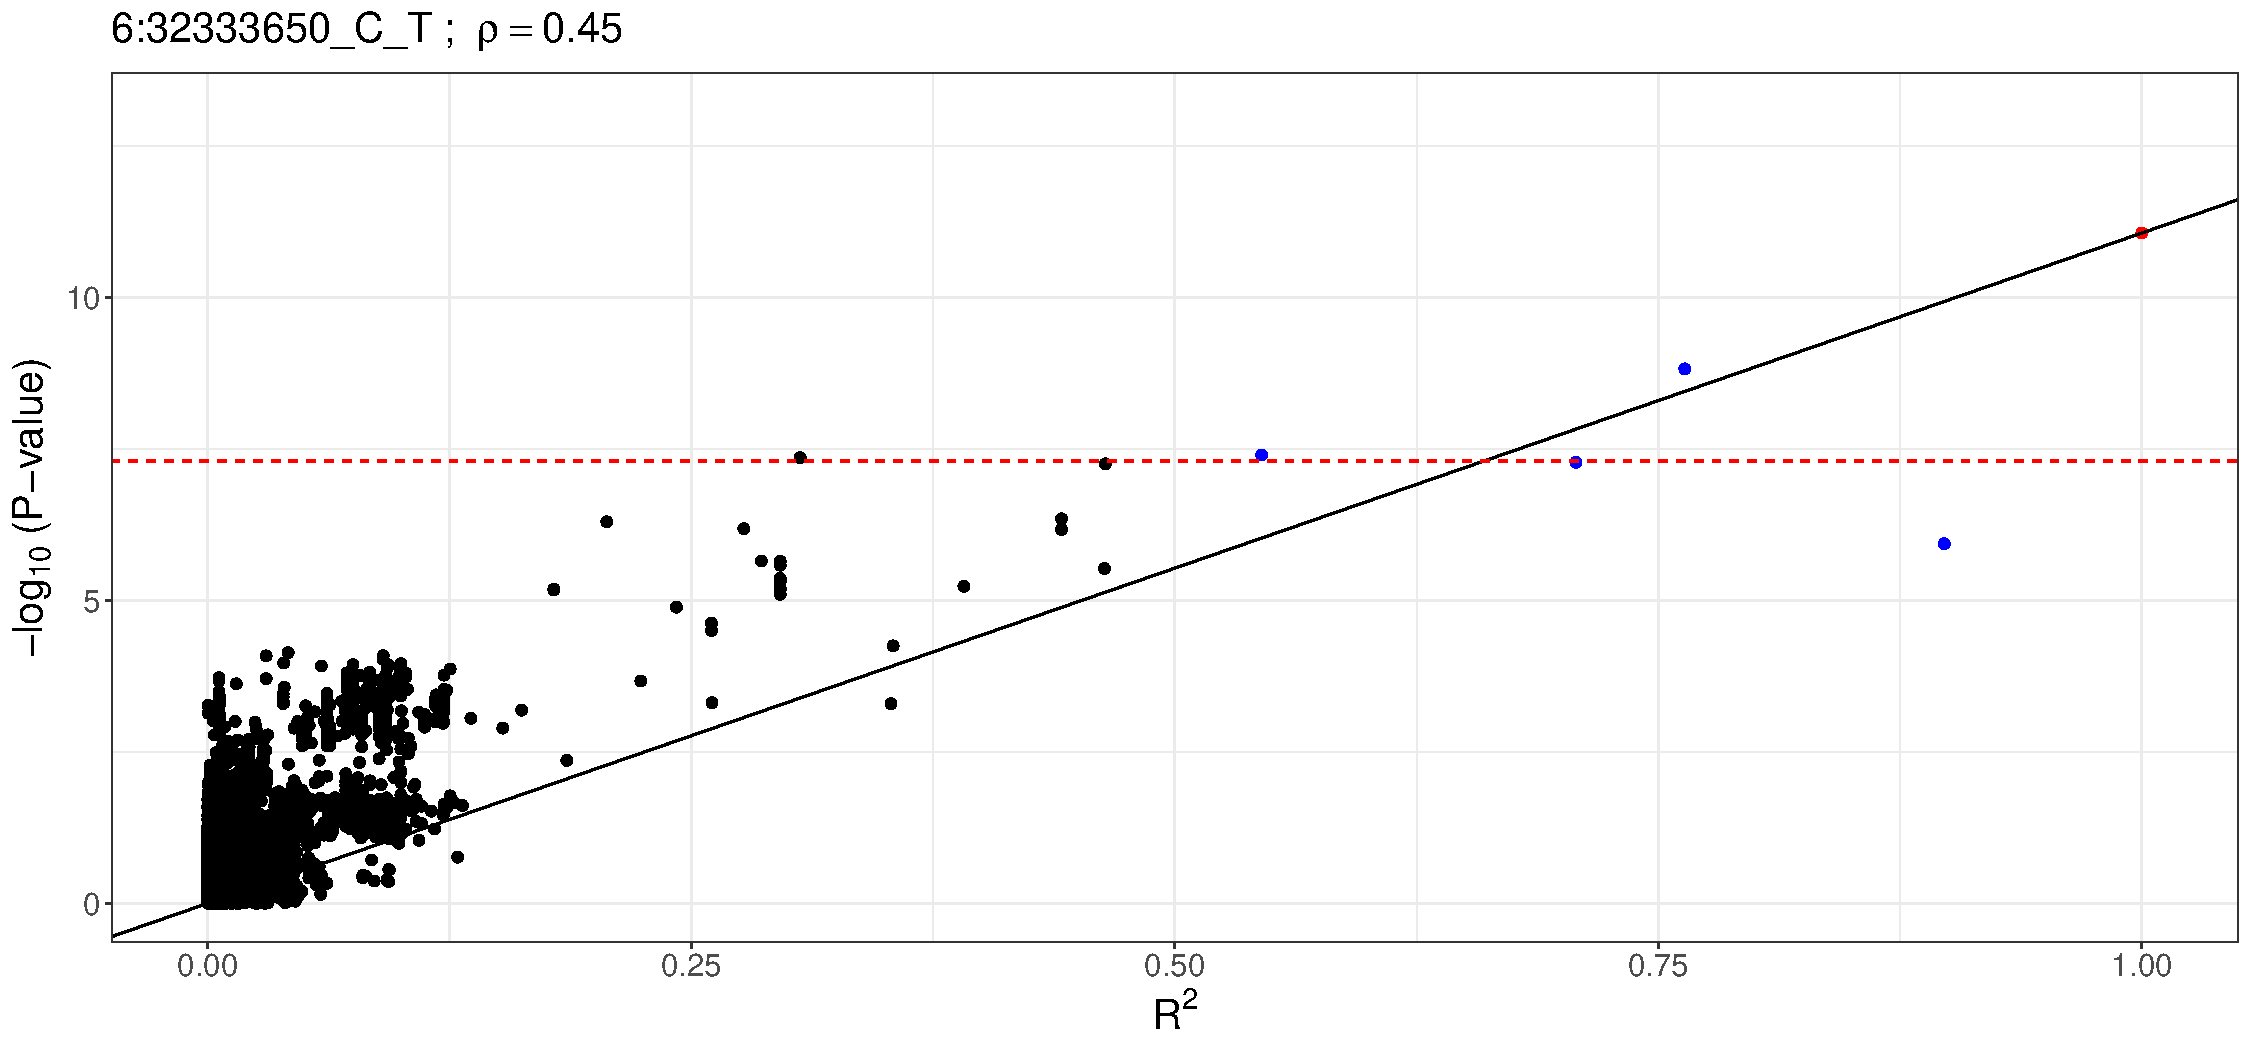
\includegraphics[width=1.0\textwidth]{fig3}
      \caption[Figure]{Association P-value for all variants in a 1mbp window around rs115378818 (P-value < $5\times10^{-4}$) on the x-axis, and $R^{2}$ of variants with the index variant on the y-axis (derived from 1000GP). Horizontal red-line indicates the genome-wide significance threshold (P-value = $5\times10^{-8}$).}
      \label{fig:ld_pval_plot}
      \end{figure}


    \subsection{Association at 6p21.32 is robust to more severe pCD+ definitions}


The IBD-BR provides information about the type of perianal involvement each patient presents with. To understand the effect of different definition criteria, I investigated how the meta-analysed association signal at 6p21.32 is sensitive to different definitions of pCD+ cases in the IBD-BR. In addition to the broad-definition meta-analysis described in the previous section ($META_{broad}$), I performed a meta-analysis between UKIBDGC and IBD-BR using three additional pCD+ definitions that have an increasingly severe impact on patients: pCD+ as abscess or simple or complex fistula only ($META_{abscfist}$), as simple or complex fistula only ($META_{fist}$), and as complex fistula only ($META_{complexfist}$). 

\begin{figure}[H] 
  \centering    
  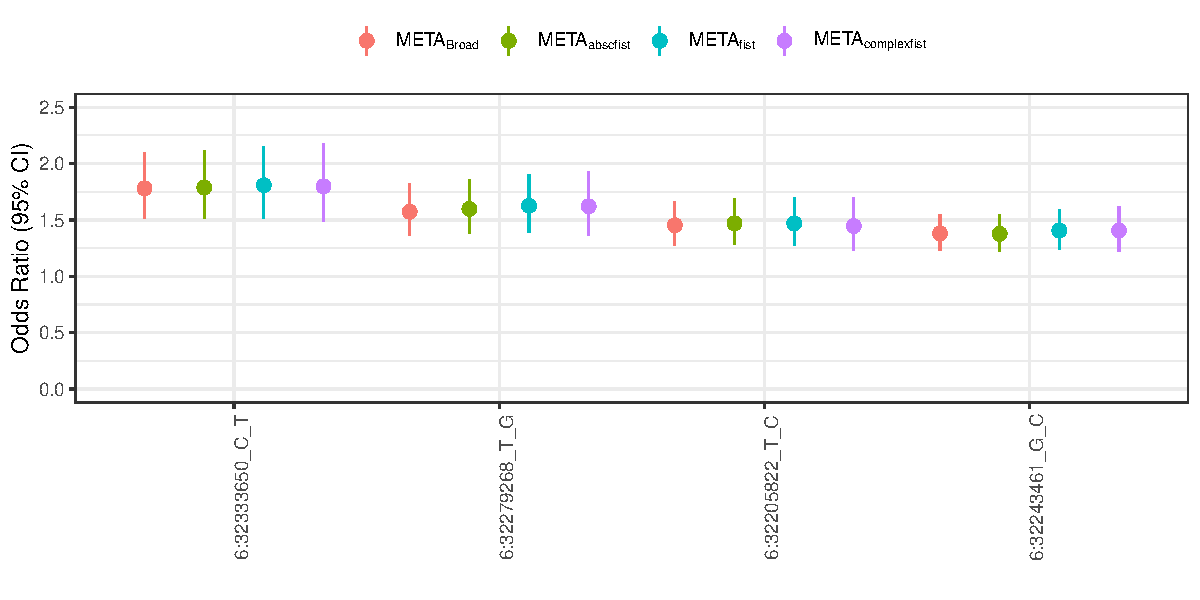
\includegraphics[width=1.0\textwidth]{pcd_def_or_plot}
  \caption[Figure]{Odds ratios of all four genome-wide significant SNPs in pCD cohorts defined with different case inclusion criteria.}
  \label{fig:pcd_def_or_plot}
  \end{figure}


I compared the effect sizes of the four-genome-wide significant SNPs and found that none of them exhibited heterogeneity of effect sizes across the different pCD definition meta-analyses ($P_{het}$ > 0.01). Additionally, I compared the association statistic between different definitions. Since the stricter definitions resulted in a reduction in the number of pCD+ cases, a proportional decrease in association test statistic ($\chi^{2}$) may also be expected. Under the hypothesis that the stricter-definition meta-analyses are simply a random subset of $META_{broad}$, the $\chi^{2}$  observed in any definition meta-analysis should match $\chi^{2}$ from $META_{broad}$ adjusted for the reduction in sample size (I will refer to this as $\chi^{2}_{Broad,n}$; see Methods for how this adjustment was performed). \\

In a 1mbp window centred around the index variant, I compared the $\chi^{2}$ statistics observed in each of the three stricter-definition meta-analyses to $\chi^{2}_{Broad,N}$. All four genome-wide significant variants achieved the expected association in the stricter definition meta-analyses. For example, rs115378818 remained genome-wide significant in $META_{fist}$ despite the decrease in sample size (1,234 fewer pCD+ cases; observed P-value=$2.2\times10^{-11}$; broad-definition P-value adjusted for sample size=$3\times10^{-11}$; Figure \ref{fig:meta_def_comparison}). More broadly, across all variants in 6p21.32, I observed strong correlation between observed $\chi^{2}$ in the stricter-definition meta-analyses and $\chi^{2}_{Broad,n}$, which shows the robustness of the association signal against different definitions of pCD+ cases in IBD-BR ($META_{abscfist}$=0.95; $META_{fist}$=0.92,$META_{complexfist}$=0.84). 

%%%%%%%%%%%%%%%%%%%%%%%%%%%%%%%%%%%%%%%%%
%FIGURE SOURCE: /lustre/scratch123/hgi/mdt2/projects/ibdgwas_ukibdgc/oe2/scripts/compare_chi_squared.R
%%%%%%%%%%%%%%%%%%%%%%%%%%%%%%%%%%%%%%%%%
\begin{figure}[H] 
  \centering    
  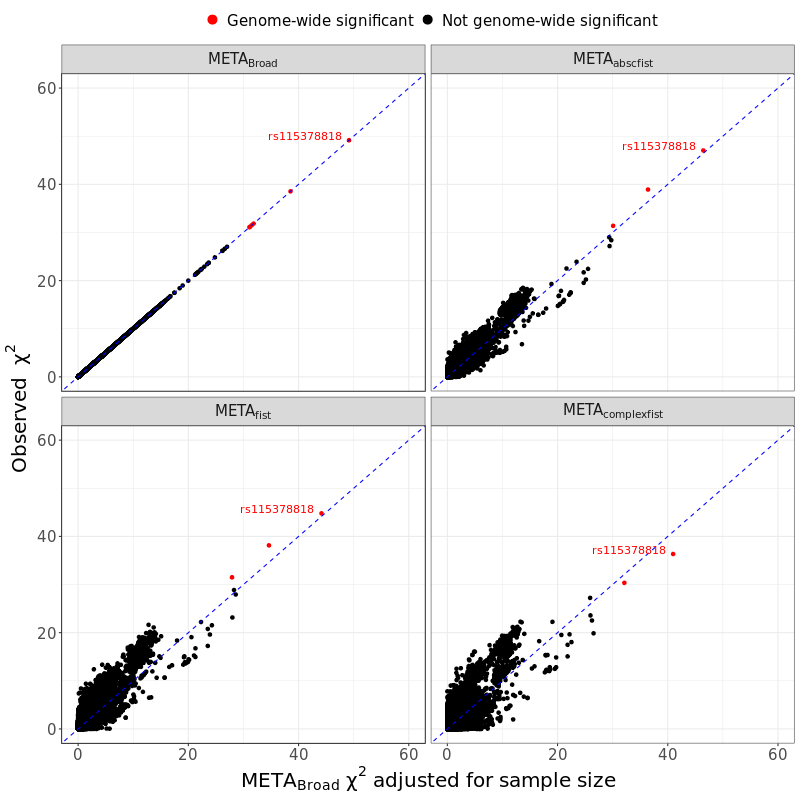
\includegraphics[width=0.8\textwidth]{Vector/meta_chisq_plot}
  \caption[Figure]{Association P-value for all variants in a 1mbp window around rs115378818 (P-value < $5\times10^{-4}$) on the x-axis, and $R^{2}$ of variants with the index variant rs115378818 on the y-axis (derived from 1000GP). The blue line indicates the line that passess through the points (0,0) and ($\chi^{2}_{Broad,n}$,$\chi^{2}_{observed}$).}
  \label{fig:meta_def_comparison}
  \end{figure}
\subsection{pCD is associated with HLA allele DRB1*01:03}
The MHC region is known to be highly polymorphic and to exhibit long-range LD patterns, which often span several hundred kbps. This makes the mapping of MHC associations to effector genes challenging \cite{Matzaraki2017-za}. To this end, HLA imputation based on genotyped variants can aid the interpretation of genome-wide significant hits in the MHC locus. HLA genes are broadly divided into class I and class II genes \cite{Marsh2010-mq}. Both classes of genes are responsible for presenting antigens to T lymphocytes and natural killer cells via antigen-presenting cells in order to initiate an innate and adaptive immune response \cite{Shiina2009-wt}. Due to the extensive polymorphism of the MHC regions, groups of HLA alleles are categorised in HLA groups which are referenced using a 2-digit naming system \cite{hla-nomenclature} (2-digit reolution; which I will refer to as \textit{allele group}). Two additional digits may be used to reference the specific HLA allele \cite{hla-nomenclature-4digit} (4-digit reolution; which I will refer to as \textit{specific allele}). 

To identify which HLA allele is associated with pCD, I performed association analyses between pCD status and class I and II HLA alleles, both at the allele group and specific allele levels (2-digit and 4-digit resolutions; see Methods for how HLA imputation was performed). Similar to the genome-wide association analysis, I performed the HLA association analyses separetely for IBD-BR and UKIBDGC and subsequently meta-analysed the summary statistics (effect sizes and standard errors). \\

None of the tested HLA alleles achieved genome-wide significance (P-value < $5\times10^{-8}$) within the cohorts or in the meta-analysis. At the allele group level, DRB1*01 had the strongest association. At a specific allele level, HLA-DRB1*01:03 had the most significant association, and had a stronger association compared to its allele group ($P_{DRB1*01:03}=1.8\times10^{-6}$; $P_{DRB1*01}=1.4\times10^{-3}$). I tested both dominant and additive modes of inheritance and found that the dominant model achieved better model fit at both the allele group and specific allele levels ($AIC_{dominant} < AIC_{additive}$; Table \ref{table:hla_allele_assoc}). 
\begin{table}[H]
  
  \centering\begingroup\fontsize{9}{10}\selectfont
  \caption{Top HLA allele associations with pCD status. Both allele groups (2-digit resolution; first two rows) and specific alleles (4-digit resolution; third and fourth rows) are shown. Meta-analysed P-values and odds ratios between UKIBDGC and IBD-BR cohorts are shown (with their 95\% confidence intervals). Both dominant and additive modes of inheritance  for  DRB1*01 and DRB1*01:03 were tested. Akaike Information Content (AIC), a measure of model fit, is shown in the last theree columns for each of the three constituent cohorts, and shows a better fit for the dominant model (lower AIC).}
  \label{table:hla_allele_assoc}
  \begin{tabular}[t]{|l|l|l|l|l|l|l|}
  \hline
  HLA Allele & Inheritance & Odds Ratio & P-value & AIC (IBDBR) & AIC (HCE) & AIC (GWAS1)\\
  \hline
  DRB1*01 & Dominant & 1.2 (1.1 - 1.3) & 9.4e-04 & 9127.887 & 3901.092 & 1783.907\\
  \hline
  DRB1*01 & Additive & 1.1 (1.1 - 1.2) & 1.5e-03 & 9128.485 & 3901.413 & 1783.907\\
  \hline
  DRB1*01:03 & Dominant & 1.6 (1.3 - 1.9) & 5.3e-07 & 9122.007 & 3651.987 & 1615.647\\
\hline
DRB1*01:03 & Additive & 1.5 (1.3 - 1.8) & 1.8e-06 & 9122.825 & 3653.500 & 1615.647\\
\hline
  \end{tabular}
  \endgroup{}
  \end{table}
\subsubsection{Conditioning association signal on DRB1*01:03}
I then asked if the DRB1*01:03 association with pCD accounted for the genome-wide significant locus at 6p21.32. Linking the two associations can explain which HLA allele the genome-wide significant hit may map to. To this end, I repeated the association tests for all variants in the locus, including DR1*01:03 as a covariate. Additionally, I repeated the HLA allele association test conditioning on the index variant in the locus to understand if the DRB*01:03 association is completely accounted for by the index variant. Similar to the GWAS and the HLA allele association tests, I also analysed the different cohorts separately and then meta-analysed the effect sizes and standard errors.\\


After conditioning on the index variant rs115378818, I did not observe an association with DRB1*01:03, indicating that the  DRB1*01:03 association is completely accounted for by the index variant ($P_{DRB1*01:03|rs115378818}$=0.61). Conversely, DRB1*01:03 did not completely account for the rs115378818 association. When I conditioned the rs115378818 association on DRB1*01:03, the index variant remained nominally associated with pCD ($P_{rs115378818}=8.6\times10^{-12}$ and  $P_{rs115378818|DRB1*01:03}=1.1\times10^{-5}$; Figure \ref{fig:residual_assoc_plot}). Taken together, this evidence suggests that  DRB1*01:03 is only nominally associated with pCD and that it only partly explains the observed genome-wide association signal. 

 
\begin{figure}[H] 
  \centering    
  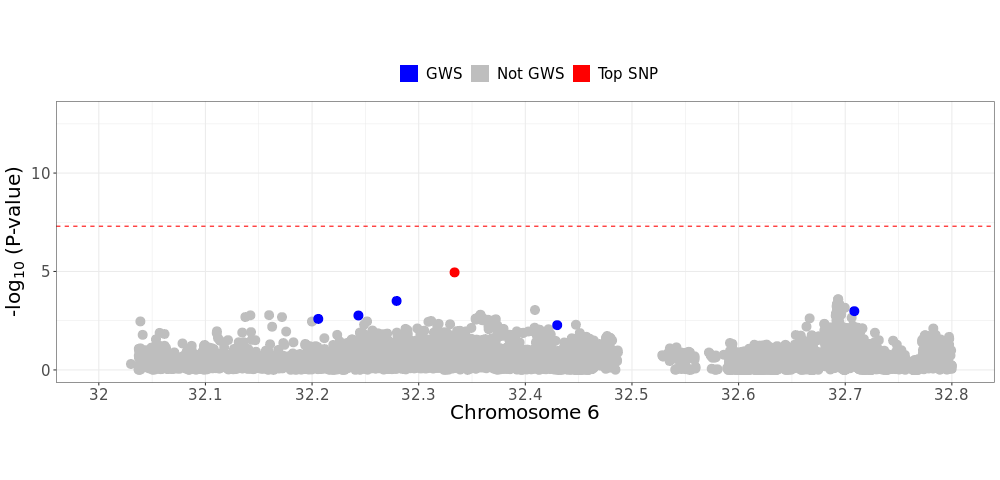
\includegraphics[width=0.7\textwidth]{Vector/cond_regional_assoc_plot}
  \caption[Figure]{Residual association signal after including DRB1*01:03 as a covariate. Blue points represent variants with a genome-wide significant association in the model that does not include DRB1:01*03. The red point indicates rs115378818 (index variant).}
  \label{fig:residual_assoc_plot}
  \end{figure}

  
\section{Discussion}
In this chapter, I have used two IBD cohorts (UKIBDGC and IBD-BR) with rich clinical data to describe the clinical characteristics of pCD and identify genetic variants associated with pCD risk. With a total of 12,897 individuals, this meta-analysis represents one of the largest pCD GWAS studies to date \cite{Akhlaghpour2023-jw}. Although others have attempted to identify pCD-associated loci, none of the studies have found genome-wide significant hits \cite{Akhlaghpour2023-jw,Kaur2016-ut}. The most recent pCD study by Akhlaghpour et al. identified a Complement Factor B (\textit{CFB}) missense variant that was nominally associated with pCD risk (rs4151651; P-value=$9.35\times10^{-6}$). \textit{CFB} is part of the alternative pathway responsible for the activation of the complement system, an innate immune subsystem that improves the ability of phagocytic cells to clear pathogens \cite{Huang2002-of,Goring2009-cs}. Functional follow-up work showed that the \textit{CFB} missense variant impairs the phagocytic ability of macrophages. This impaired phagocytic capability was hypothesised to impact the ability of the immune system to fight bacterial strains found in the fistulas of CD patients. Although this study established a plausible factor that may contribute to pCD risk, a more complete picture of its pathogenesis is needed.\\


In an attempt to fill the gap in our understanding of pCD pathogenesis, I performed a meta-analysis of two pCD cohorts, with a total of 3,967 pCD+ cases and 8,930 pCD- controls. I identified a genome-wide significant locus in the highly polymorphic Major Histocompatibility Locus (MHC) at 6p21.32 that was associated with pCD risk (index variant rs115378818). Additionally, my post-GWAS checks have reasonably confirmed the veracity of this association. Furthermore, the assocaition signal revealed by our meta-analysis is likely distinct from the \textit{CFB} association. First, rs115378818 and rs4151651 are in weak LD ($R^{2}$=0.24). Second, upon conditioning on the \textit{CFB} signal (rs114969413; $R^{2}$ with index variant $=0.99$), rs115378818 remained nominally associated suggesting that the \textit{CFB} does not completely account for it ($P_{rs115378818|rs114969413}$=$2.1\times10^{-6}$; Figure \ref{fig:cond_mcgovern}), and showing that our genome-wide significant variant represents a novel pCD-associated locus. \\

\begin{figure}
  \centering    
  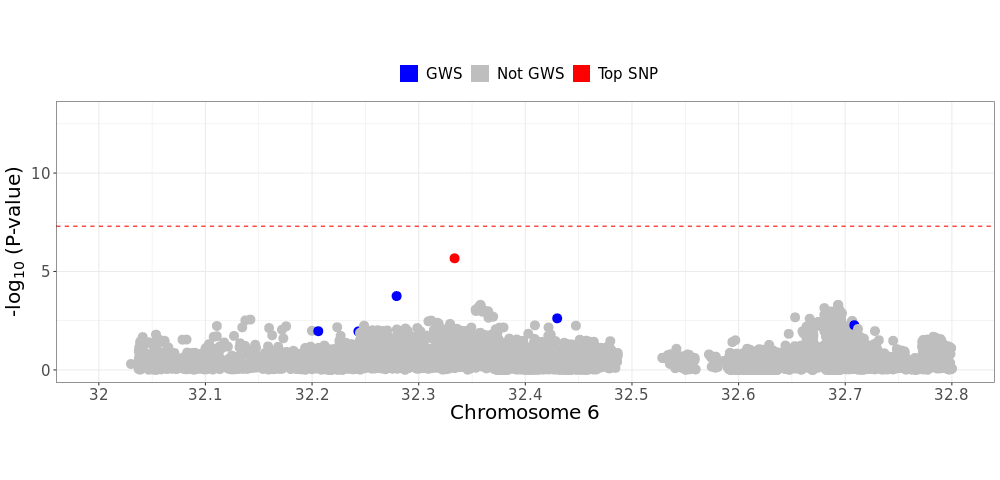
\includegraphics[width=0.7\textwidth]{Vector/cond_mcgovern_regional_assoc_plot}
  \caption[Figure]{Residual association signal after including  rs114969413 (a \textit{CFB} locus variant) as a covariate. Blue points represent variants with a genome-wide significant association in the model that does not include rs114969413. The red point indicates rs115378818 (index variant).}
  \label{fig:cond_mcgovern}
  \end{figure}
  
  Despite our ability to identify a novel association, case heterogeneity remains an important limitation of this study. Akhlaghpour et al. have also noted that a potentially heterogeneous composition of their cohorts may have decreased their power to detect genome-wide associations with pCD. Their cohorts, similar to ours, may have had patients with milder forms of pCD such as skin tags and ulcer. Therefore, I tested the association of our locus with pCD+ cases redefined with increasingly severe criteria and found that the genome-wide significant association was robust to different case definitions. However, the heterogeneity of case definition may still have decreased our power to detect \textit{additional} pCD-associated loci. In this study, a more refined definition of pCD+ as fistulising pCD was hampered by the unavailability of more granular data on the specific pCD manifestations in the UKIBDGC cohort. It remains to be seen if larger sample sizes can overcome the heterogeneity in case definition and identify more pCD-associated loci. Increasing power will not only identify more pCD-associated loci, but it will also give us a more complete understanding of the pathogenesis of pCD, and may implicate biological pathways that are targeted by pCD-associated genetic variation. \\


  Nonetheless, the finding that HLA-DRB1*01:03 may explain the genome-wide association signal is a promising starting point. HLA-DRB1*01:03 has been previously shown to be associated with colonic Crohn's disease, ulcerative colitis risk \cite{Goyette2015-xx,Cleynen2016-ha} and rheumatoid arthritis (RA) \cite{Klimenta2019-be}. However, several avenues should be explored to identify which HLA alleles completely account for the genome-wide significant association. Several reasons may explain the incomplete association of HLA-DRB*1:03 with pCD. First, the association signal at 6p21.32 may be explained by multiple HLA alleles, and therefore conditioning on a single HLA allele cannot completely explain the 6p21.32 signal. The highly polymorphic nature of most HLA genes often makes it difficult to completely attribute disease risk to a single HLA allele. This has been previously observed for rheumatoid arthritis (RA), where several \textit{HLA-DRB1} alleles confer risk to RA \cite{Van_Drongelen2017-dh}. Second, multiple \textit{HLA-DRB1} alleles with slight differences in their amino acid sequences, especially in the peptide binding regions, have different affinities to antigens being presented to T-cells \cite{Wang2022-hk}. Therefore, testing the pCD association with multiple HLA-DRB1 alleles that share the same amino acid sequences might better account for the pCD signal \cite{Molineros2019-mu}. Interestingly, Raychaudhuri et al. found that only three amino acid positions in a predictive model of RA risk provided identical prediction to a model that included all \textit{HLA-DRB1} allleles \cite{Raychaudhuri2012-em}. Therefore, an important follow-up to my work should explore the association of HLA-DRB1 alleles with pCD at the amino acid level. \\

Finally, it is important that future studies do not consider pCD as an isolated disease. The broad clinical phenotyping of IBD-BR showed lower drug intake, higher prevalence of extraintestinal manifestations, and higher prevalence of rectal CD in pCD+ patients. These observations naturally pose a question about how these disease characteristics relate to pCD. A plausible explanation is that these clinical characteristics are simply manifestations of what is collectively termed "severe CD". It is still important however to understand how severe CD drives these seemingly unrelated manifestations. For example, is there common pathogenesis, or genetic predisposition that drives all these manifestations, including pCD? In this regard, my univariate pCD meta-analysis is limited. Future studies should quantify the genetic correlation between pCD and disease severity and location, extraintestinal manifestations, and drug response. Furthermore, multivariate GWAS methods should be employed to identify shared and distinct genetic factors driving each of these manifesations. The observation that clusters of disorders have common as well as distinct genetic factors has been previously shown to further our understanding of multiple groups of disorders such as psychiatric disorders \cite{Grotzinger2019-bt}. \\





Literature about pCD pathogenesis largely attributes the development of fistlising CD to the theory of epithelial-to-mesenchymal transformation of epithelial cells. With the ongoing growth of IBD-BR, and with more genotyped CD participants, a more nuanced understanding of which dysregulated pathways give rise to pCD risk, and whether or not these pathways corroborate the EMT theory of pCD pathogenesis is increasingly attainable.


% \section{Second section of the third chapter}
% and here I write more \dots

% \section{The layout of formal tables}
% This section has been modified from ``Publication quality tables in \LaTeX*''
%  by Simon Fear.

% The layout of a table has been established over centuries of experience and 
% should only be altered in extraordinary circumstances. 

% When formatting a table, remember two simple guidelines at all times:

% \begin{enumerate}
%   \item Never, ever use vertical rules (lines).
%   \item Never use double rules.
% \end{enumerate}

% These guidelines may seem extreme but I have
% never found a good argument in favour of breaking them. For
% example, if you feel that the information in the left half of
% a table is so different from that on the right that it needs
% to be separated by a vertical line, then you should use two
% tables instead. Not everyone follows the second guideline:

% There are three further guidelines worth mentioning here as they
% are generally not known outside the circle of professional
% typesetters and subeditors:

% \begin{enumerate}\setcounter{enumi}{2}
%   \item Put the units in the column heading (not in the body of
%           the table).
%   \item Always precede a decimal point by a digit; thus 0.1
%       {\em not} just .1.
%   \item Do not use `ditto' signs or any other such convention to
%       repeat a previous value. In many circumstances a blank
%       will serve just as well. If it won't, then repeat the value.
% \end{enumerate}

% A frequently seen mistake is to use `\textbackslash begin\{center\}' \dots `\textbackslash end\{center\}' inside a figure or table environment. This center environment can cause additional vertical space. If you want to avoid that just use `\textbackslash centering'

